\documentclass[]{book}
\usepackage{lmodern}
\usepackage{amssymb,amsmath}
\usepackage{ifxetex,ifluatex}
\usepackage{fixltx2e} % provides \textsubscript
\ifnum 0\ifxetex 1\fi\ifluatex 1\fi=0 % if pdftex
  \usepackage[T1]{fontenc}
  \usepackage[utf8]{inputenc}
\else % if luatex or xelatex
  \ifxetex
    \usepackage{mathspec}
  \else
    \usepackage{fontspec}
  \fi
  \defaultfontfeatures{Ligatures=TeX,Scale=MatchLowercase}
\fi
% use upquote if available, for straight quotes in verbatim environments
\IfFileExists{upquote.sty}{\usepackage{upquote}}{}
% use microtype if available
\IfFileExists{microtype.sty}{%
\usepackage{microtype}
\UseMicrotypeSet[protrusion]{basicmath} % disable protrusion for tt fonts
}{}
\usepackage[margin=1in]{geometry}
\usepackage{hyperref}
\hypersetup{unicode=true,
            pdftitle={Data Visualization with R},
            pdfauthor={Claudia A Engel},
            pdfborder={0 0 0},
            breaklinks=true}
\urlstyle{same}  % don't use monospace font for urls
\usepackage{natbib}
\bibliographystyle{apalike}
\usepackage{color}
\usepackage{fancyvrb}
\newcommand{\VerbBar}{|}
\newcommand{\VERB}{\Verb[commandchars=\\\{\}]}
\DefineVerbatimEnvironment{Highlighting}{Verbatim}{commandchars=\\\{\}}
% Add ',fontsize=\small' for more characters per line
\usepackage{framed}
\definecolor{shadecolor}{RGB}{248,248,248}
\newenvironment{Shaded}{\begin{snugshade}}{\end{snugshade}}
\newcommand{\KeywordTok}[1]{\textcolor[rgb]{0.13,0.29,0.53}{\textbf{#1}}}
\newcommand{\DataTypeTok}[1]{\textcolor[rgb]{0.13,0.29,0.53}{#1}}
\newcommand{\DecValTok}[1]{\textcolor[rgb]{0.00,0.00,0.81}{#1}}
\newcommand{\BaseNTok}[1]{\textcolor[rgb]{0.00,0.00,0.81}{#1}}
\newcommand{\FloatTok}[1]{\textcolor[rgb]{0.00,0.00,0.81}{#1}}
\newcommand{\ConstantTok}[1]{\textcolor[rgb]{0.00,0.00,0.00}{#1}}
\newcommand{\CharTok}[1]{\textcolor[rgb]{0.31,0.60,0.02}{#1}}
\newcommand{\SpecialCharTok}[1]{\textcolor[rgb]{0.00,0.00,0.00}{#1}}
\newcommand{\StringTok}[1]{\textcolor[rgb]{0.31,0.60,0.02}{#1}}
\newcommand{\VerbatimStringTok}[1]{\textcolor[rgb]{0.31,0.60,0.02}{#1}}
\newcommand{\SpecialStringTok}[1]{\textcolor[rgb]{0.31,0.60,0.02}{#1}}
\newcommand{\ImportTok}[1]{#1}
\newcommand{\CommentTok}[1]{\textcolor[rgb]{0.56,0.35,0.01}{\textit{#1}}}
\newcommand{\DocumentationTok}[1]{\textcolor[rgb]{0.56,0.35,0.01}{\textbf{\textit{#1}}}}
\newcommand{\AnnotationTok}[1]{\textcolor[rgb]{0.56,0.35,0.01}{\textbf{\textit{#1}}}}
\newcommand{\CommentVarTok}[1]{\textcolor[rgb]{0.56,0.35,0.01}{\textbf{\textit{#1}}}}
\newcommand{\OtherTok}[1]{\textcolor[rgb]{0.56,0.35,0.01}{#1}}
\newcommand{\FunctionTok}[1]{\textcolor[rgb]{0.00,0.00,0.00}{#1}}
\newcommand{\VariableTok}[1]{\textcolor[rgb]{0.00,0.00,0.00}{#1}}
\newcommand{\ControlFlowTok}[1]{\textcolor[rgb]{0.13,0.29,0.53}{\textbf{#1}}}
\newcommand{\OperatorTok}[1]{\textcolor[rgb]{0.81,0.36,0.00}{\textbf{#1}}}
\newcommand{\BuiltInTok}[1]{#1}
\newcommand{\ExtensionTok}[1]{#1}
\newcommand{\PreprocessorTok}[1]{\textcolor[rgb]{0.56,0.35,0.01}{\textit{#1}}}
\newcommand{\AttributeTok}[1]{\textcolor[rgb]{0.77,0.63,0.00}{#1}}
\newcommand{\RegionMarkerTok}[1]{#1}
\newcommand{\InformationTok}[1]{\textcolor[rgb]{0.56,0.35,0.01}{\textbf{\textit{#1}}}}
\newcommand{\WarningTok}[1]{\textcolor[rgb]{0.56,0.35,0.01}{\textbf{\textit{#1}}}}
\newcommand{\AlertTok}[1]{\textcolor[rgb]{0.94,0.16,0.16}{#1}}
\newcommand{\ErrorTok}[1]{\textcolor[rgb]{0.64,0.00,0.00}{\textbf{#1}}}
\newcommand{\NormalTok}[1]{#1}
\usepackage{longtable,booktabs}
\usepackage{graphicx,grffile}
\makeatletter
\def\maxwidth{\ifdim\Gin@nat@width>\linewidth\linewidth\else\Gin@nat@width\fi}
\def\maxheight{\ifdim\Gin@nat@height>\textheight\textheight\else\Gin@nat@height\fi}
\makeatother
% Scale images if necessary, so that they will not overflow the page
% margins by default, and it is still possible to overwrite the defaults
% using explicit options in \includegraphics[width, height, ...]{}
\setkeys{Gin}{width=\maxwidth,height=\maxheight,keepaspectratio}
\IfFileExists{parskip.sty}{%
\usepackage{parskip}
}{% else
\setlength{\parindent}{0pt}
\setlength{\parskip}{6pt plus 2pt minus 1pt}
}
\setlength{\emergencystretch}{3em}  % prevent overfull lines
\providecommand{\tightlist}{%
  \setlength{\itemsep}{0pt}\setlength{\parskip}{0pt}}
\setcounter{secnumdepth}{5}
% Redefines (sub)paragraphs to behave more like sections
\ifx\paragraph\undefined\else
\let\oldparagraph\paragraph
\renewcommand{\paragraph}[1]{\oldparagraph{#1}\mbox{}}
\fi
\ifx\subparagraph\undefined\else
\let\oldsubparagraph\subparagraph
\renewcommand{\subparagraph}[1]{\oldsubparagraph{#1}\mbox{}}
\fi

%%% Use protect on footnotes to avoid problems with footnotes in titles
\let\rmarkdownfootnote\footnote%
\def\footnote{\protect\rmarkdownfootnote}

%%% Change title format to be more compact
\usepackage{titling}

% Create subtitle command for use in maketitle
\newcommand{\subtitle}[1]{
  \posttitle{
    \begin{center}\large#1\end{center}
    }
}

\setlength{\droptitle}{-2em}
  \title{Data Visualization with R}
  \pretitle{\vspace{\droptitle}\centering\huge}
  \posttitle{\par}
  \author{Claudia A Engel}
  \preauthor{\centering\large\emph}
  \postauthor{\par}
  \predate{\centering\large\emph}
  \postdate{\par}
  \date{Last updated: April 27, 2018}

\usepackage{booktabs}
\usepackage{amsthm}
\makeatletter
\def\thm@space@setup{%
  \thm@preskip=8pt plus 2pt minus 4pt
  \thm@postskip=\thm@preskip
}
\makeatother

\usepackage{amsthm}
\newtheorem{theorem}{Theorem}[chapter]
\newtheorem{lemma}{Lemma}[chapter]
\theoremstyle{definition}
\newtheorem{definition}{Definition}[chapter]
\newtheorem{corollary}{Corollary}[chapter]
\newtheorem{proposition}{Proposition}[chapter]
\theoremstyle{definition}
\newtheorem{example}{Example}[chapter]
\theoremstyle{definition}
\newtheorem{exercise}{Exercise}[chapter]
\theoremstyle{remark}
\newtheorem*{remark}{Remark}
\newtheorem*{solution}{Solution}
\begin{document}
\maketitle

{
\setcounter{tocdepth}{1}
\tableofcontents
}
\chapter*{Prerequisites and
Preparations}\label{prerequisites-and-preparations}
\addcontentsline{toc}{chapter}{Prerequisites and Preparations}

To get the most out of this workshop you should have:

\begin{itemize}
\tightlist
\item
  a \textbf{basic knowledge} of R and/or be familiar with the topics
  covered in the \href{https://cengel.github.io/R-intro/}{Introduction
  to R}.
\item
  have a recent version of \href{https://cran.r-project.org/}{R} and
  \href{https://www.rstudio.com/}{RStudio} installed.
\item
  have installed the \href{http://tidyverse.org/}{\texttt{tidyverse}}
  package.
\end{itemize}

\textbf{Recommended}:

\begin{itemize}
\tightlist
\item
  Create a new RStudio project \texttt{R-data-viz} in a new folder
  \texttt{R-data-viz} and download both CSV files into a subdirectory
  called \texttt{data}:

  \begin{itemize}
  \tightlist
  \item
    Download \texttt{MS\_stops.csv} from here:
    \url{https://github.com/cengel/R-data-viz/raw/master/data/MS_stops.csv}
  \item
    Download \texttt{MS\_county\_stops.csv} from here:
    \url{https://github.com/cengel/R-data-viz/raw/master/data/MS_county_stops.csv}
  \item
    If you have your working directory set to \texttt{R-data-viz} which
    contains a folder called \texttt{data} you can copy, paste, and run
    the following lines in R:
  \end{itemize}
\end{itemize}

\begin{Shaded}
\begin{Highlighting}[]
\KeywordTok{download.file}\NormalTok{(}\StringTok{"https://github.com/cengel/R-data-viz/raw/master/data/MS_stops.csv"}\NormalTok{, }
              \StringTok{"data/MS_stops.csv"}\NormalTok{)}

\KeywordTok{download.file}\NormalTok{(}\StringTok{"https://github.com/cengel/R-data-viz/raw/master/data/MS_stops_by_county.csv"}\NormalTok{, }
              \StringTok{"data/MS_stops_by_county.csv"}\NormalTok{)}
\end{Highlighting}
\end{Shaded}

\begin{itemize}
\tightlist
\item
  Open up a new R Script file \texttt{R-data-viz.R} for the code you'll
  create during the workshop.
\end{itemize}

\section*{References}\label{references}
\addcontentsline{toc}{section}{References}

Chang, W. (2012): R Graphics Cookbook.
\href{https://stanford.idm.oclc.org/login?url=http://proquest.safaribooksonline.com/?uiCode=stanford\&xmlId=9781449363086}{Stanford
only online access}

Murrell, P. (2012): R Graphics, 2nd ed.
\href{https://stanford.idm.oclc.org/login?url=http://proquest.safaribooksonline.com/?uiCode=stanford\&xmlId=9781439831779}{Stanford
only online access}

Rahlf, T (2017): Data Visualisation with R.
\url{http://www.springer.com/us/book/9783319497501}

Wickham, H. (2016): ggplot2: Elegant Graphics for Data Analysis. 2nd ed.
\url{http://link.springer.com/book/10.1007/978-3-319-24277-4}

\section*{Acknowledgements}\label{acknowledgements}
\addcontentsline{toc}{section}{Acknowledgements}

Part of the materials for this tutorial are adapted from
\url{http://datacarpentry.org} and \url{http://softwarecarpentry.org}.

Data sample taken from \url{https://openpolicing.stanford.edu/}

\chapter{\texorpdfstring{Data Visualization with
\texttt{ggplot2}}{Data Visualization with ggplot2}}\label{data-visualization-with-ggplot2}

\begin{quote}
Learning Objectives

\begin{itemize}
\tightlist
\item
  Bind a data frame to a plot
\item
  Select variables to be plotted and variables to define the
  presentation such as size, shape, color, transparency, etc. by
  defining aesthetics (\texttt{aes})
\item
  Add a graphical representation of the data in the plot (points, lines,
  bars) adding ``geoms'' layers
\item
  Produce univariate plots, barplots and histograms, area plots,
  boxplots, and line plots, using ggplot.
\item
  Produce bivariate plots, like scatter plots, hex plots, stacked bars,
  and bivariate line charts using ggplot.
\item
  Modify the aesthetics for the entire plot as well as for individual
  ``geoms'' layers
\item
  Modify plot elements (labels, text, scale, orientation)
\item
  Group observations by a factor variable
\item
  Break up plot into multiple panels (facetting)
\item
  Apply ggplot themes and create and apply customized themes
\item
  Save a plot created by ggplot as an image
\end{itemize}
\end{quote}

\begin{center}\rule{0.5\linewidth}{\linethickness}\end{center}

\section{\texorpdfstring{What is
\textbf{\texttt{ggplot2}}}{What is ggplot2}}\label{what-is-ggplot2}

There are three main plotting systems in R, the
\href{https://www.statmethods.net/graphs/index.html}{base plotting}
system, the
\href{https://www.statmethods.net/advgraphs/trellis.html}{lattice}
package, and the
\href{https://www.statmethods.net/advgraphs/ggplot2.html}{ggplot2}
package.

Here we will introduce the \texttt{ggplot2} package, which has recently
soared in popularity. \texttt{ggplot} allows you to create graphs for
univariate and multivariate numerical and categorical data in a
straightforward manner. It also allows for easy grouping and
conditioning. It can generate complex plots create high quality graphics
for publication.

\texttt{ggplot} is built on
\href{https://stanford.idm.oclc.org/login?url=http://www.myilibrary.com?id=46066}{Leland
Wilkinson's The Grammar of Graphics}, the idea that any plot can be
expressed from the same set of components:

\begin{itemize}
\tightlist
\item
  a data set,
\item
  a coordinate system,
\item
  and a set of geoms--the visual representation of data points.
\end{itemize}

The key to understanding \texttt{ggplot} is thinking about a figure in
layers. This idea may be familiar to you if you have used image editing
programs like Photoshop, Illustrator, or Inkscape.

\textbf{\texttt{ggplot2}} provides a programmatic interface for
specifying what variables to plot, how they are displayed, and what the
general visual properties are, so we only need minimal changes if the
underlying data change or if we decide to change from a bar plot to a
scatterplot. This helps in creating plots quickly with minimal amounts
of adjustments and tweaking.

\texttt{ggplot} generally likes data in the `long' format: i.e., a
column for every dimension, and a row for every observation. Well
structured data will save you lots of time when making figures with
ggplot.

\section{\texorpdfstring{Plotting with
\textbf{\texttt{ggplot2}}}{Plotting with ggplot2}}\label{plotting-with-ggplot2}

We start by loading the required package. Note that
\textbf{\texttt{ggplot2}} is part of the collection of the
\href{https://www.tidyverse.org}{\textbf{\texttt{tidyverse}} packages}.

\begin{Shaded}
\begin{Highlighting}[]
\KeywordTok{library}\NormalTok{(ggplot2)}
\end{Highlighting}
\end{Shaded}

Next we load the data into R:

\begin{Shaded}
\begin{Highlighting}[]
\NormalTok{stops_county <-}\StringTok{ }\KeywordTok{read.csv}\NormalTok{(}\StringTok{'data/MS_stops_by_county.csv'}\NormalTok{)}
\end{Highlighting}
\end{Shaded}

These data are a small subset extracted from the
\href{https://openpolicing.stanford.edu}{openpolicing.stanford.edu}
dataset and contain traffic stops by police aggregated for each county
in Missisippi. Let's take a look at the data.

\begin{Shaded}
\begin{Highlighting}[]
\KeywordTok{head}\NormalTok{(stops_county)}
\KeywordTok{str}\NormalTok{(stops_county)}
\end{Highlighting}
\end{Shaded}

The table contains two variables which represent for each county, and
for both white and black, the ratio of drivers stopped out of the total
population over 18: \texttt{pct\_black\_stopped} and
\texttt{pct\_white\_stopped}. In order to see if there is any `bias' we
can plot the two values against each other and see if they line up at a
45 degree angle.

\texttt{ggplot} graphics are built step by step by adding new elements
(layers) using the \texttt{+} sign.

To build a \texttt{ggplot} we need to:

\begin{itemize}
\tightlist
\item
  bind the plot to a specific data frame using the \texttt{data}
  argument
\end{itemize}

\begin{Shaded}
\begin{Highlighting}[]
\KeywordTok{ggplot}\NormalTok{(}\DataTypeTok{data =}\NormalTok{ stops_county)}
\end{Highlighting}
\end{Shaded}

\begin{itemize}
\tightlist
\item
  define aesthetics (\texttt{aes}), by selecting the variables to be
  plotted and the variables to define the presentation such as plotting
  size, shape color, etc.
\end{itemize}

\begin{Shaded}
\begin{Highlighting}[]
\KeywordTok{ggplot}\NormalTok{(}\DataTypeTok{data =}\NormalTok{ stops_county, }\KeywordTok{aes}\NormalTok{(}\DataTypeTok{x =}\NormalTok{ pct_black_stopped, }\DataTypeTok{y =}\NormalTok{ pct_white_stopped))}
\end{Highlighting}
\end{Shaded}

\begin{itemize}
\tightlist
\item
  add ``geoms'' -- a graphical representation of the data in the plot
  (points, lines, bars). To add a geom to the plot use \texttt{+}
  operator
\end{itemize}

\begin{Shaded}
\begin{Highlighting}[]
\KeywordTok{ggplot}\NormalTok{(}\DataTypeTok{data =}\NormalTok{ stops_county, }\KeywordTok{aes}\NormalTok{(}\DataTypeTok{x =}\NormalTok{ pct_black_stopped, }\DataTypeTok{y =}\NormalTok{ pct_white_stopped)) }\OperatorTok{+}
\StringTok{  }\KeywordTok{geom_point}\NormalTok{()}
\end{Highlighting}
\end{Shaded}

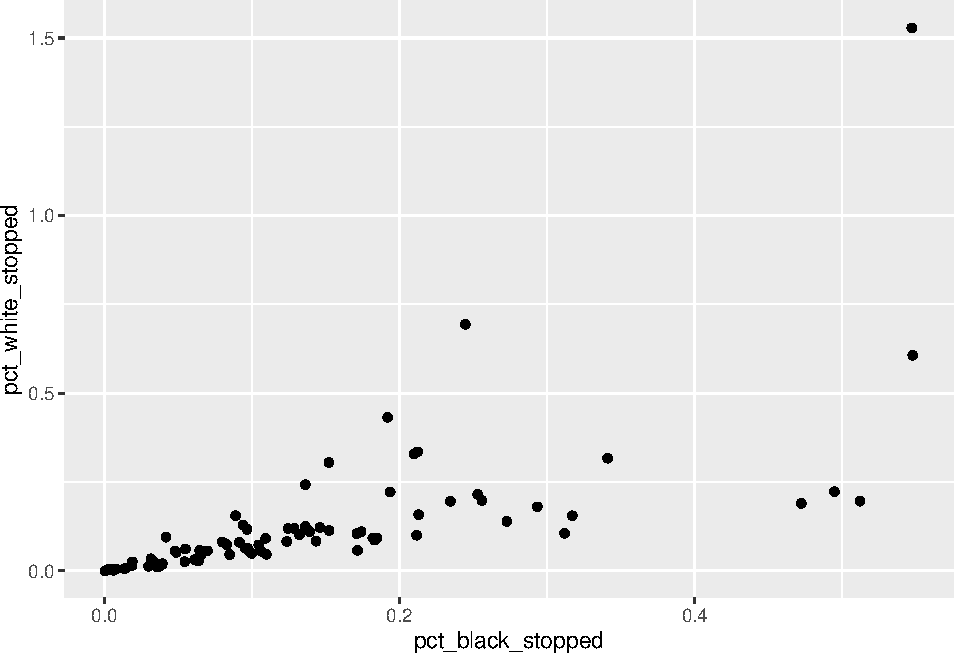
\includegraphics[width=0.7\linewidth]{R-data-viz_files/figure-latex/first-ggplot-1}

The \texttt{+} in the \textbf{\texttt{ggplot2}} package is particularly
useful because it allows you to modify existing \texttt{ggplot} objects.
This means you can easily set up plot ``templates'' and conveniently
explore different types of plots, so the above plot can also be
generated with code like this:

\begin{Shaded}
\begin{Highlighting}[]
\CommentTok{# Assign plot to a variable}
\NormalTok{MS_plot <-}\StringTok{ }\KeywordTok{ggplot}\NormalTok{(}\DataTypeTok{data =}\NormalTok{ stops_county, }\KeywordTok{aes}\NormalTok{(}\DataTypeTok{x =}\NormalTok{ pct_black_stopped, }\DataTypeTok{y =}\NormalTok{ pct_white_stopped))}

\CommentTok{# Draw the plot}
\NormalTok{MS_plot }\OperatorTok{+}\StringTok{ }\KeywordTok{geom_point}\NormalTok{()}
\end{Highlighting}
\end{Shaded}

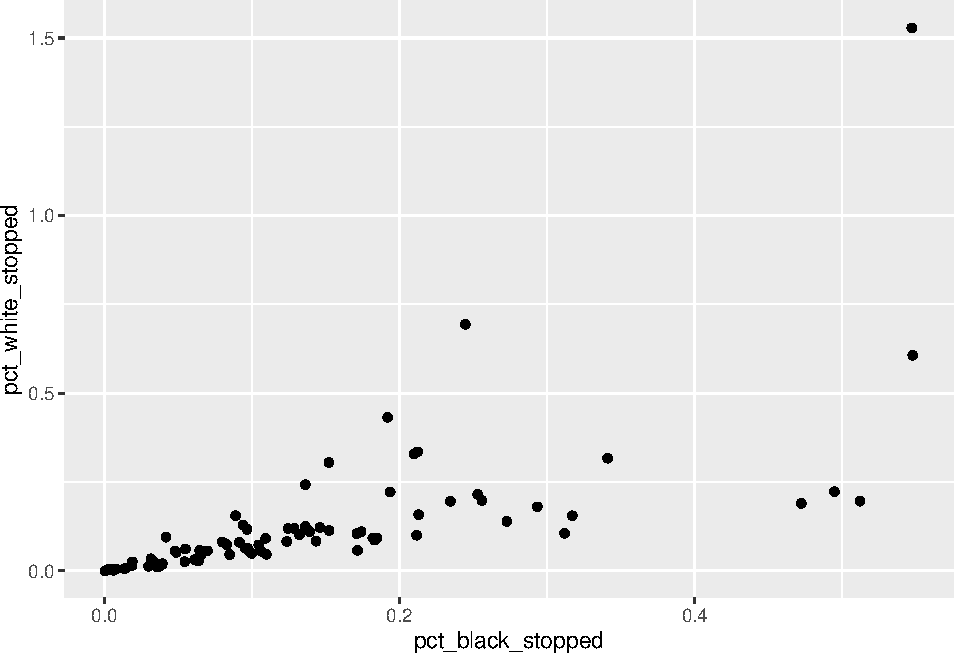
\includegraphics{R-data-viz_files/figure-latex/first-ggplot-with-plus-1.pdf}

Notes:

\begin{itemize}
\tightlist
\item
  Any parameters you set in the \texttt{ggplot()} function can be seen
  by any geom layers that you add (i.e., these are universal plot
  settings). This includes the x and y axis you set up in
  \texttt{aes()}.
\item
  Any parameters you set in a \texttt{geom\_*()} function are treated
  independently of (and possibly override) the settings defined globally
  in the \texttt{ggplot()} function.
\item
  Geoms are plotted in the order they are added after each \texttt{+},
  that means geoms last added will display on top of prior geoms.
\item
  The \texttt{+} sign used to add layers \textbf{must be placed at the
  end of each line} containing a layer. If, instead, the \texttt{+} sign
  is added in the line before the other layer, \textbf{\texttt{ggplot2}}
  will not add the new layer and will return an error message.
\end{itemize}

\begin{Shaded}
\begin{Highlighting}[]
\CommentTok{# this is the correct syntax for adding layers}
\NormalTok{MS_plot }\OperatorTok{+}
\StringTok{  }\KeywordTok{geom_point}\NormalTok{()}

\CommentTok{# this will not add the new layer and will return an error message}
\NormalTok{MS_plot}
  \OperatorTok{+}\StringTok{ }\KeywordTok{geom_point}\NormalTok{()}
\end{Highlighting}
\end{Shaded}

To learn more about \textbf{\texttt{ggplot}} after the workshop, you may
want to check out this
\href{https://www.rstudio.com/wp-content/uploads/2016/11/ggplot2-cheatsheet-2.1.pdf}{cheatsheet
about \textbf{\texttt{ggplot}}}.

\section{Building your plots
iteratively}\label{building-your-plots-iteratively}

Building plots with ggplot can be of great help when you engage in
exploratory data analysis. It is typically an iterative process, where
you go back and forth between your data and their graphical
representation, which helps you in the process of getting to know your
data better.

We can start modifying this plot to extract more information from it.
For instance, we can add transparency (\texttt{alpha}) to avoid
overplotting:

\begin{Shaded}
\begin{Highlighting}[]
\NormalTok{MS_plot }\OperatorTok{+}\StringTok{ }
\StringTok{  }\KeywordTok{geom_point}\NormalTok{(}\DataTypeTok{alpha =} \FloatTok{0.3}\NormalTok{)}
\end{Highlighting}
\end{Shaded}

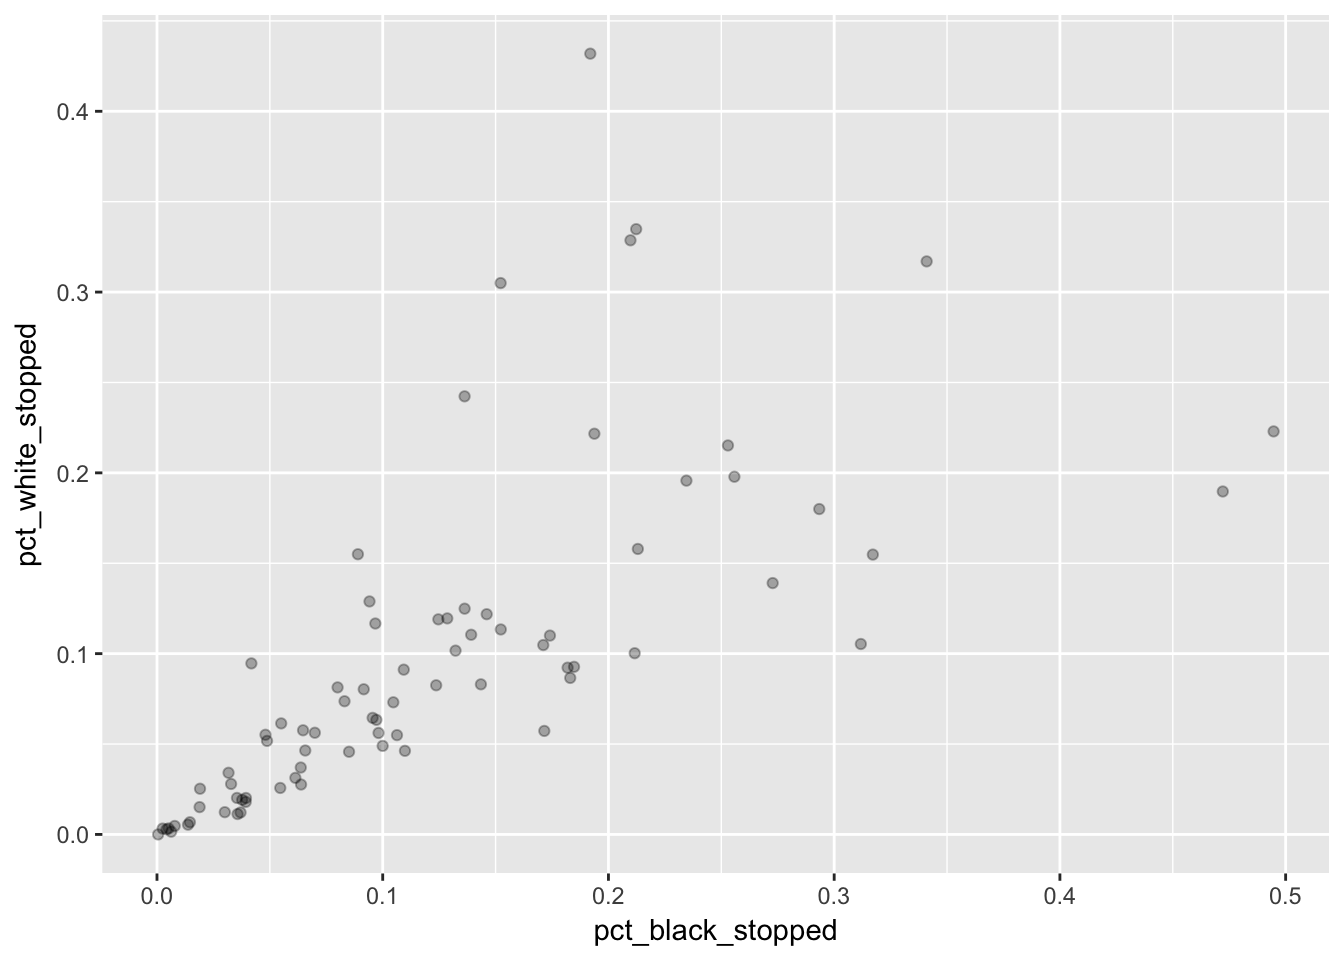
\includegraphics[width=0.7\linewidth]{R-data-viz_files/figure-latex/adding-transparency-1}

We can also add a color for all the points:

\begin{Shaded}
\begin{Highlighting}[]
\NormalTok{MS_plot }\OperatorTok{+}\StringTok{  }
\StringTok{  }\KeywordTok{geom_point}\NormalTok{(}\DataTypeTok{alpha =} \FloatTok{0.3}\NormalTok{, }\DataTypeTok{color=} \StringTok{"blue"}\NormalTok{)}
\end{Highlighting}
\end{Shaded}

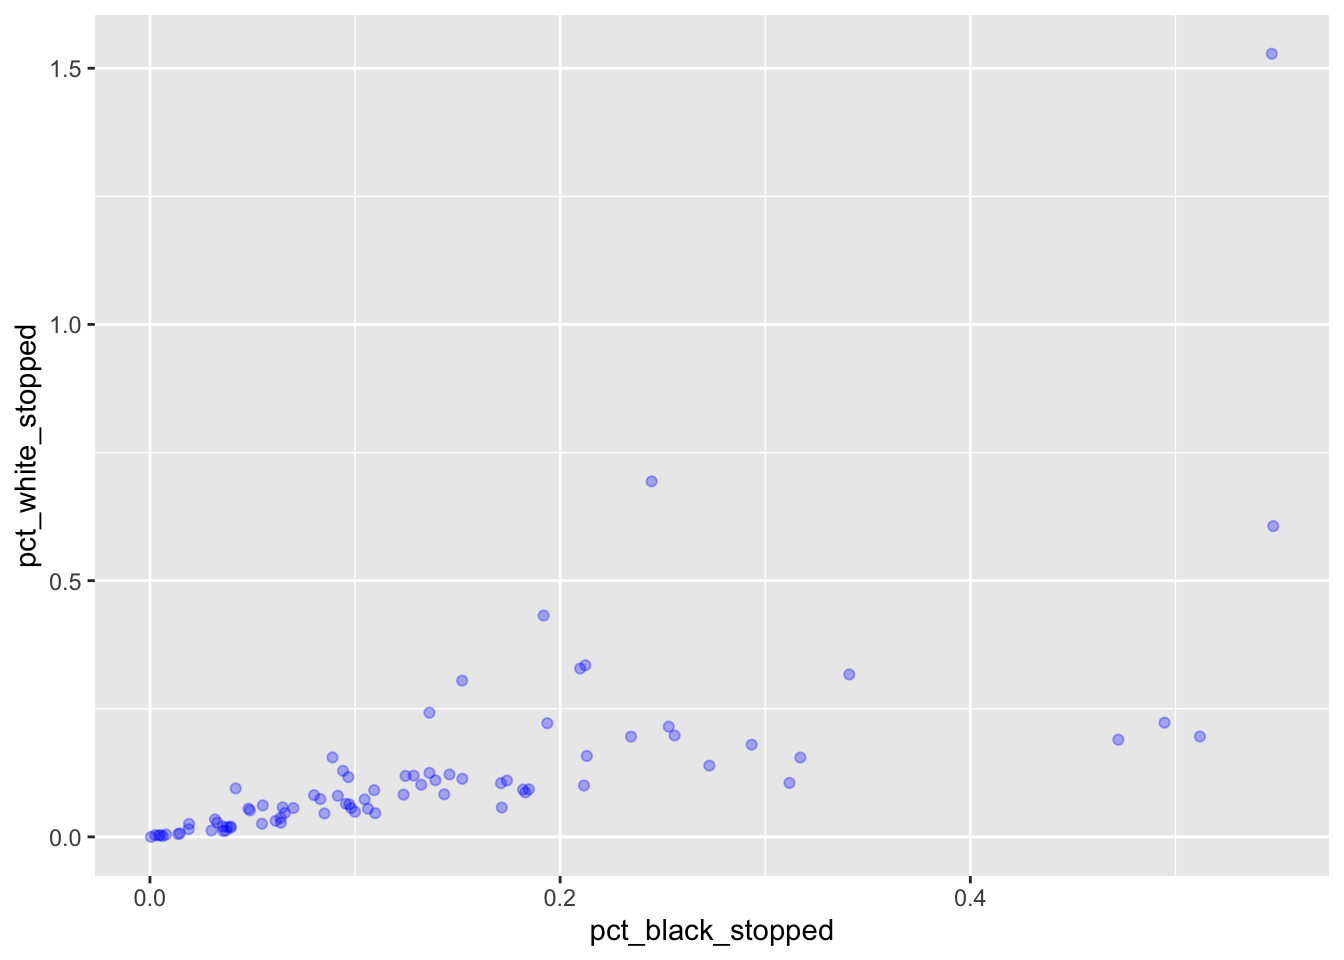
\includegraphics[width=0.7\linewidth]{R-data-viz_files/figure-latex/adding-color-1}

We can add another layer to the plot with \texttt{+}:

\begin{Shaded}
\begin{Highlighting}[]
\NormalTok{MS_plot }\OperatorTok{+}\StringTok{ }
\StringTok{  }\KeywordTok{geom_point}\NormalTok{(}\DataTypeTok{alpha =} \FloatTok{0.3}\NormalTok{, }\DataTypeTok{color=} \StringTok{"blue"}\NormalTok{) }\OperatorTok{+}
\StringTok{  }\KeywordTok{geom_abline}\NormalTok{(}\DataTypeTok{intercept =} \DecValTok{0}\NormalTok{)}
\end{Highlighting}
\end{Shaded}

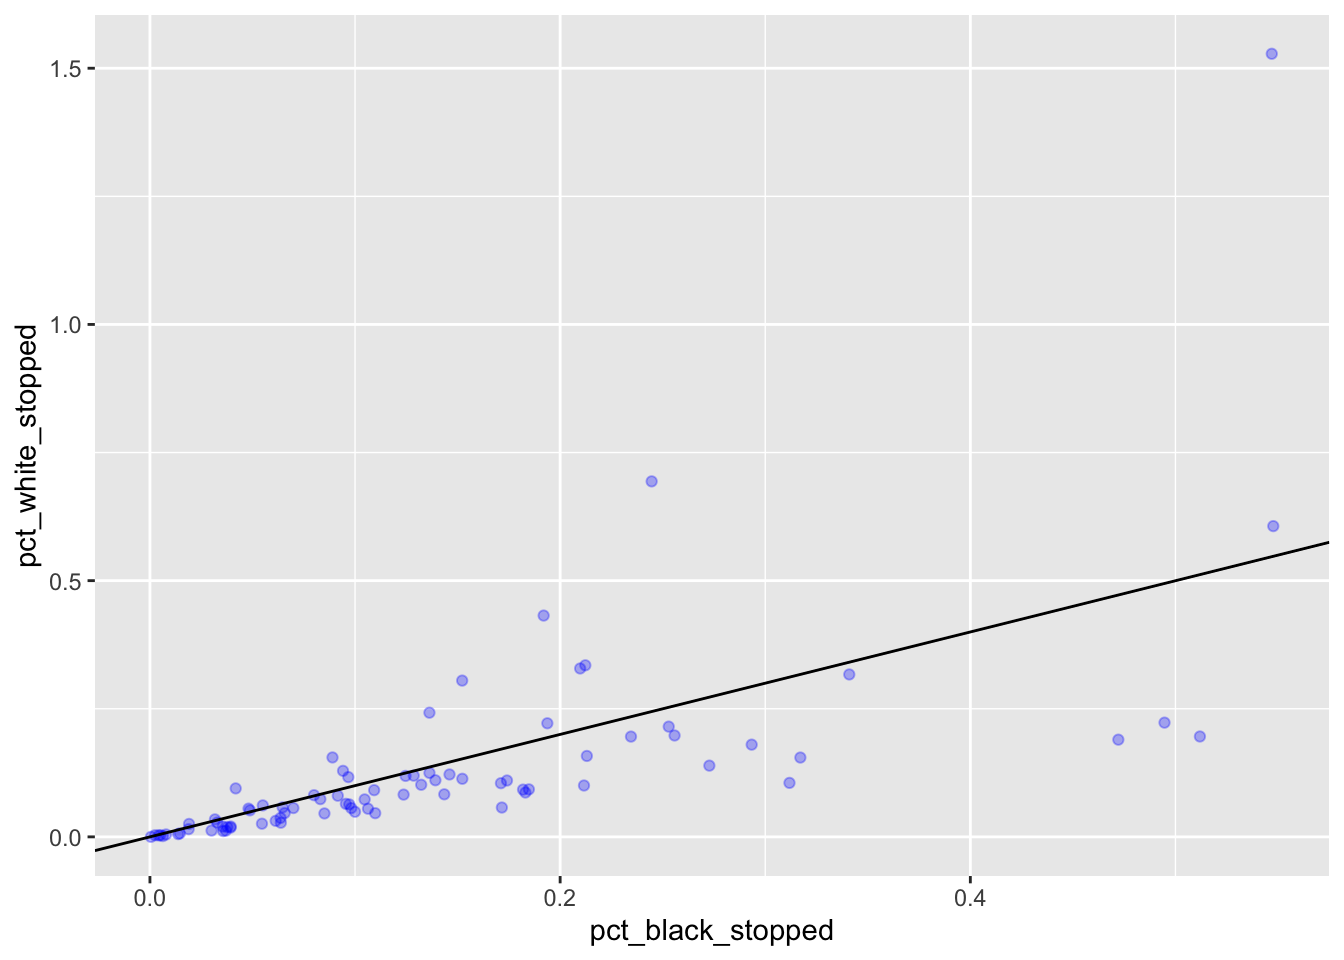
\includegraphics[width=0.7\linewidth]{R-data-viz_files/figure-latex/add-abline-1}

If we wanted to ``zoom'' into the plot, we could filter to a smaller
range of values before passing them to ggplot, but we can also tell
ggplot to only plot the x and y values for certain ranges. For this we
use \texttt{scale\_x\_continuous} and \texttt{scale\_y\_continuous}. You
will receive a message from ggplot telling you how many rows it has
removed from the plot.

\begin{Shaded}
\begin{Highlighting}[]
\NormalTok{MS_plot }\OperatorTok{+}\StringTok{ }
\StringTok{  }\KeywordTok{geom_point}\NormalTok{(}\DataTypeTok{alpha =} \FloatTok{0.3}\NormalTok{, }\DataTypeTok{color=} \StringTok{"blue"}\NormalTok{) }\OperatorTok{+}
\StringTok{  }\KeywordTok{geom_abline}\NormalTok{(}\DataTypeTok{intercept =} \DecValTok{0}\NormalTok{) }\OperatorTok{+}\StringTok{ }
\StringTok{  }\KeywordTok{scale_x_continuous}\NormalTok{(}\DataTypeTok{limits =} \KeywordTok{c}\NormalTok{(}\DecValTok{0}\NormalTok{, }\FloatTok{0.1}\NormalTok{)) }\OperatorTok{+}
\StringTok{  }\KeywordTok{scale_y_continuous}\NormalTok{(}\DataTypeTok{limits =} \KeywordTok{c}\NormalTok{(}\DecValTok{0}\NormalTok{, }\FloatTok{0.1}\NormalTok{)) }
\end{Highlighting}
\end{Shaded}

\begin{verbatim}
#> Warning: Removed 44 rows containing missing values (geom_point).
\end{verbatim}

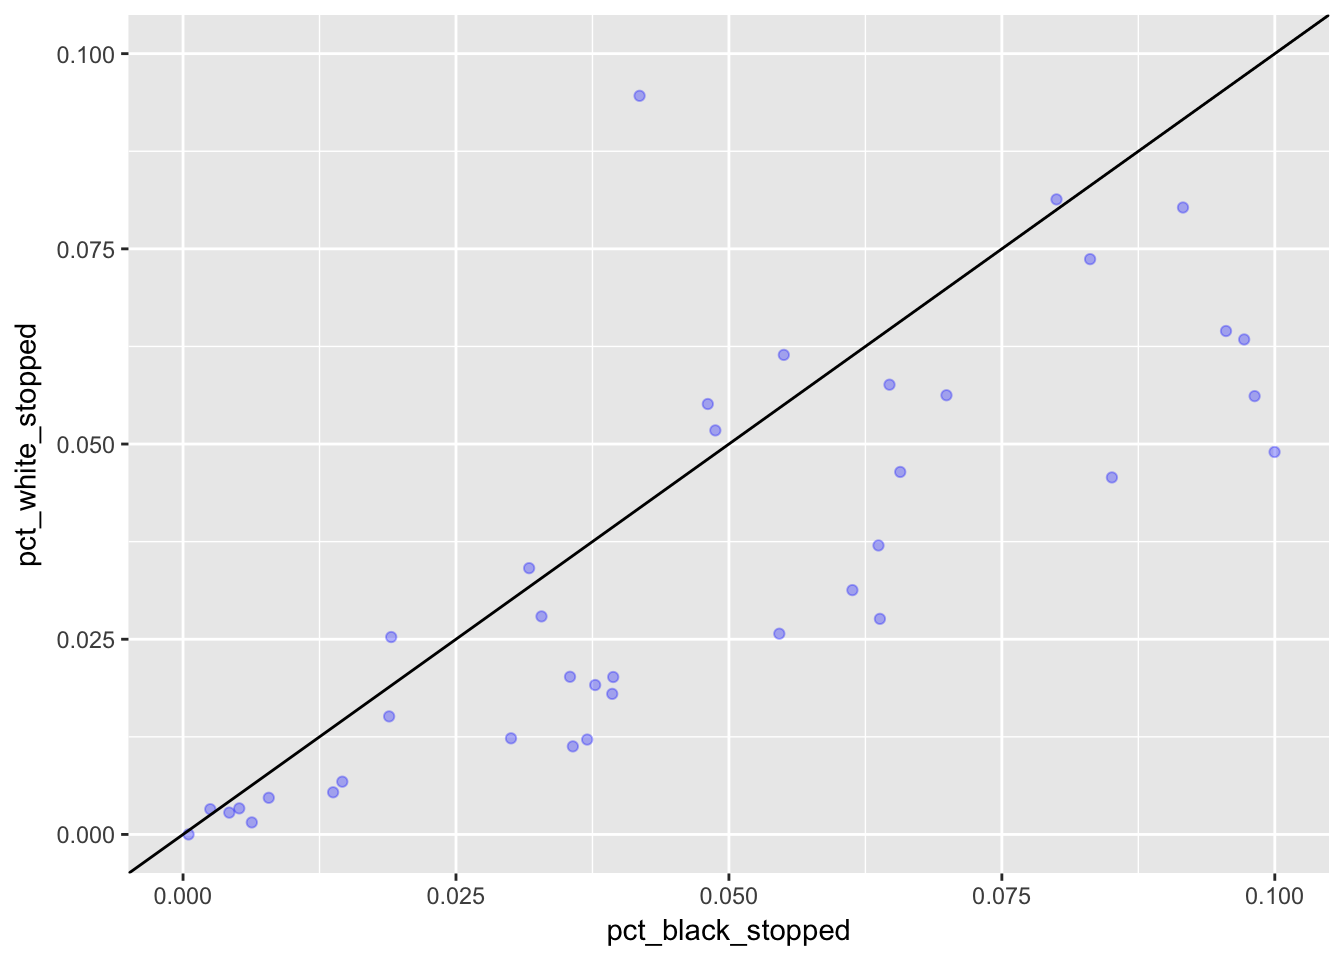
\includegraphics[width=0.7\linewidth]{R-data-viz_files/figure-latex/zoom-in-1}

\begin{quote}
Challenge

Modify the plot above to display different color for both points and
abline, and show a different range of data. How might you change the
size of the dots?
\end{quote}

Let us now use the \texttt{wb\_delta} variable (where I have subtracted
\texttt{pct\_black\_stopped} from \texttt{pct\_white\_stopped}) to
indicate bias for each of the MS counties. We can use a geom called
\texttt{geom\_col}, where heights of the bars represent values in the
data, like so:

\begin{Shaded}
\begin{Highlighting}[]
\KeywordTok{ggplot}\NormalTok{(stops_county, }\KeywordTok{aes}\NormalTok{(}\DataTypeTok{x =}\NormalTok{ county_name, }\DataTypeTok{y =}\NormalTok{ wb_delta)) }\OperatorTok{+}\StringTok{ }
\StringTok{  }\KeywordTok{geom_col}\NormalTok{()}
\end{Highlighting}
\end{Shaded}

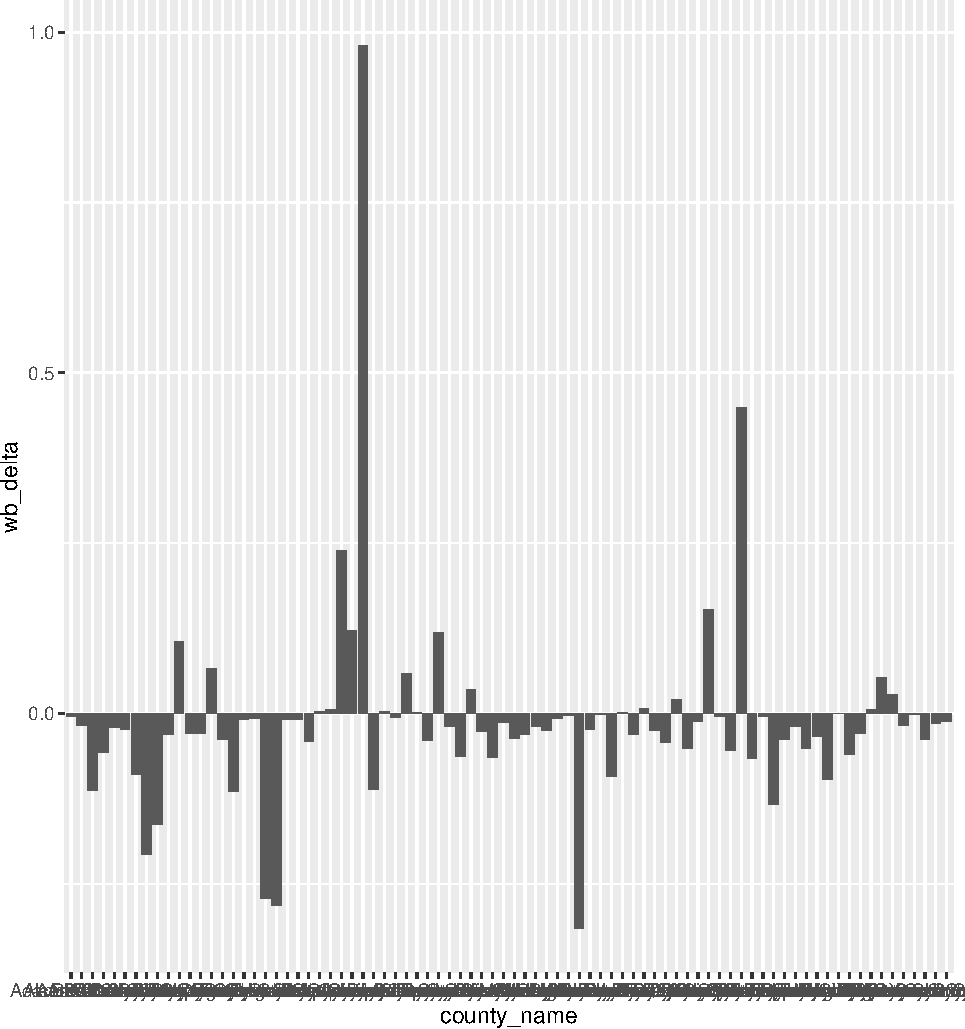
\includegraphics{R-data-viz_files/figure-latex/bias-colplot-1.pdf}

This is not very readable, so we will make some changes.

\begin{enumerate}
\def\labelenumi{\arabic{enumi}.}
\tightlist
\item
  We use coord\_flip() to switch the x and y axes and be able to read
  the county names better:
\end{enumerate}

\begin{Shaded}
\begin{Highlighting}[]
\KeywordTok{ggplot}\NormalTok{(stops_county, }\KeywordTok{aes}\NormalTok{(}\DataTypeTok{x =}\NormalTok{ county_name, }\DataTypeTok{y =}\NormalTok{ wb_delta)) }\OperatorTok{+}
\StringTok{  }\KeywordTok{geom_col}\NormalTok{() }\OperatorTok{+}\StringTok{ }
\StringTok{  }\KeywordTok{coord_flip}\NormalTok{()}
\end{Highlighting}
\end{Shaded}

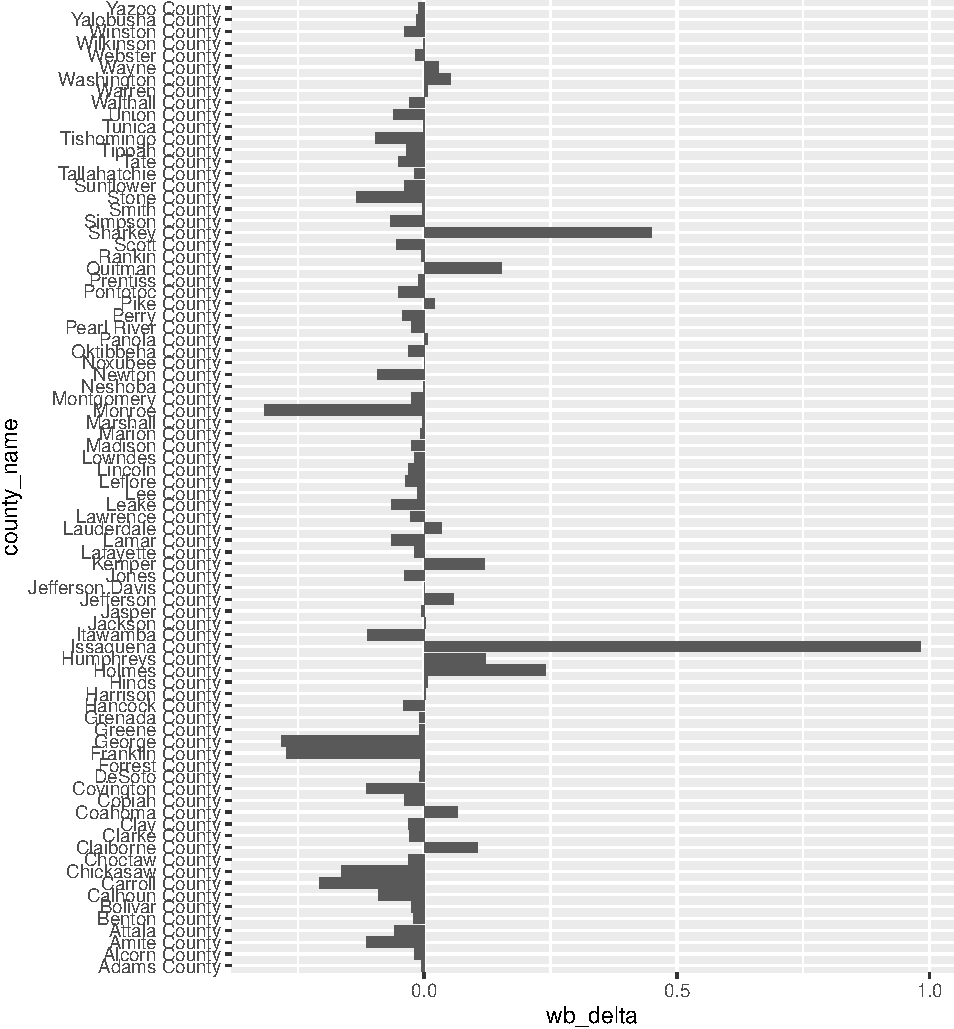
\includegraphics{R-data-viz_files/figure-latex/bias-colplot-flip-1.pdf}

\begin{enumerate}
\def\labelenumi{\arabic{enumi}.}
\setcounter{enumi}{1}
\tightlist
\item
  We order the counties (x axis) by the delta values plotted on the y
  axis. From lowest (=black bias) to highest value (=white bias).
\end{enumerate}

\begin{Shaded}
\begin{Highlighting}[]
\KeywordTok{ggplot}\NormalTok{(stops_county, }\KeywordTok{aes}\NormalTok{(}\DataTypeTok{x =} \KeywordTok{reorder}\NormalTok{(county_name, }\OperatorTok{-}\NormalTok{wb_delta), }\DataTypeTok{y =}\NormalTok{ wb_delta)) }\OperatorTok{+}
\StringTok{  }\KeywordTok{geom_col}\NormalTok{() }\OperatorTok{+}\StringTok{ }
\StringTok{  }\KeywordTok{coord_flip}\NormalTok{()}
\end{Highlighting}
\end{Shaded}

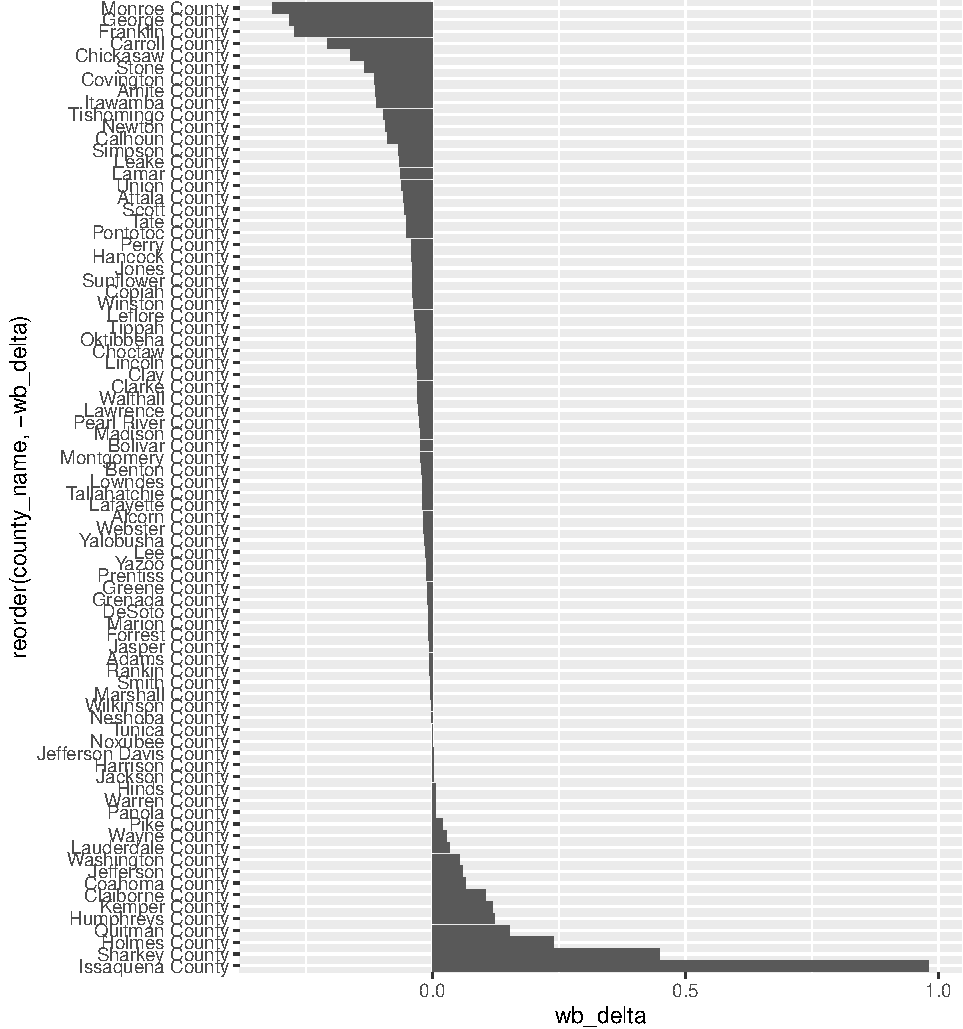
\includegraphics{R-data-viz_files/figure-latex/bias-colplot-reorder-1.pdf}

We can still improve this, but will leave it for now.

\section{Univariate distributions}\label{univariate-distributions}

For this section we will use the other dataset provided.

\begin{Shaded}
\begin{Highlighting}[]
\NormalTok{stops <-}\StringTok{ }\KeywordTok{read.csv}\NormalTok{(}\StringTok{'data/MS_stops.csv'}\NormalTok{)}
\end{Highlighting}
\end{Shaded}

It contains one entry for each traffic stop in Mississippi between 2013
and 2016.

\begin{Shaded}
\begin{Highlighting}[]
\KeywordTok{str}\NormalTok{(stops)}
\end{Highlighting}
\end{Shaded}

For distributions of discrete variables we use \texttt{geom\_bar}. It
makes the height of the bar proportional to the number of cases in each
group and counts the number of cases at each x position. If we wanted to
see how many traffic violations we have of each type could say:

\begin{Shaded}
\begin{Highlighting}[]
\KeywordTok{ggplot}\NormalTok{(stops, }\KeywordTok{aes}\NormalTok{(violation)) }\OperatorTok{+}\StringTok{ }
\StringTok{  }\KeywordTok{geom_bar}\NormalTok{()}
\end{Highlighting}
\end{Shaded}

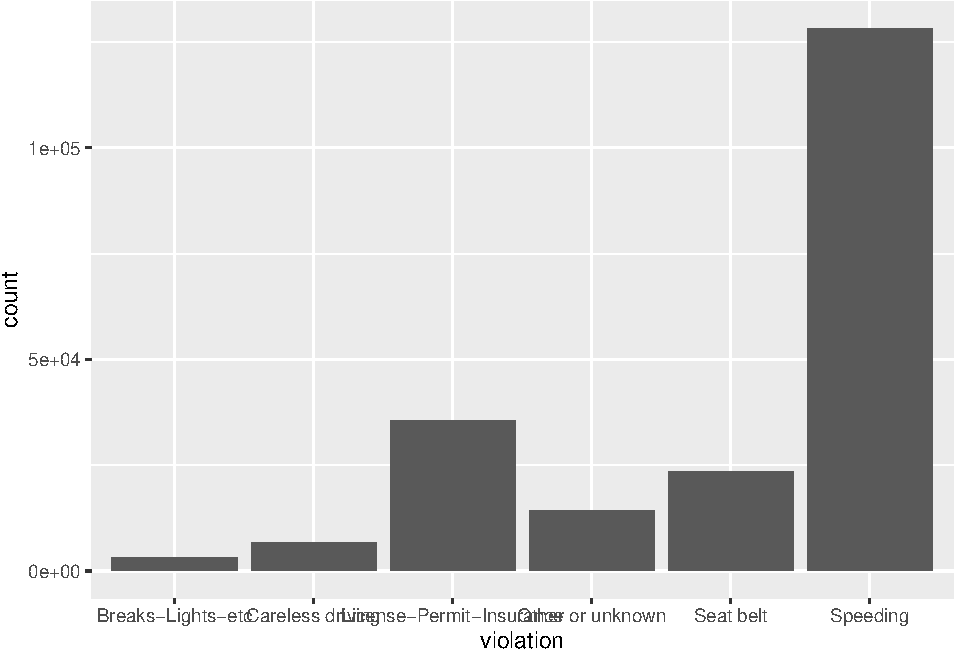
\includegraphics[width=0.7\linewidth]{R-data-viz_files/figure-latex/bar-simple-1}

We could color the bars, but instead of \texttt{color} we use
\texttt{fill}. (What happens when you use \texttt{color}?)

\begin{Shaded}
\begin{Highlighting}[]
\KeywordTok{ggplot}\NormalTok{(stops, }\KeywordTok{aes}\NormalTok{(violation)) }\OperatorTok{+}\StringTok{ }
\StringTok{  }\KeywordTok{geom_bar}\NormalTok{(}\DataTypeTok{fill =} \StringTok{"green"}\NormalTok{)}
\end{Highlighting}
\end{Shaded}

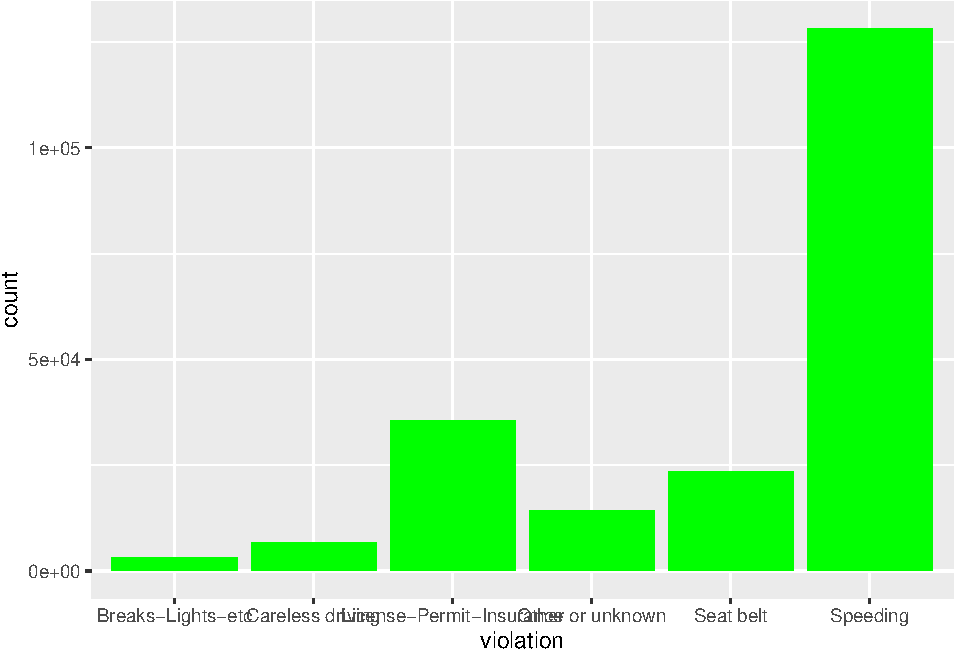
\includegraphics[width=0.7\linewidth]{R-data-viz_files/figure-latex/color-bar-simple-1}

Instead of coloring everything the same we could also color by another
category, say gender. For this we have to set the parameter within the
\texttt{aes()} function, which takes care of mapping the values to
different colors:

\begin{Shaded}
\begin{Highlighting}[]
\KeywordTok{ggplot}\NormalTok{(stops, }\KeywordTok{aes}\NormalTok{(violation)) }\OperatorTok{+}\StringTok{ }
\StringTok{  }\KeywordTok{geom_bar}\NormalTok{(}\KeywordTok{aes}\NormalTok{(}\DataTypeTok{fill =}\NormalTok{ driver_gender))}
\end{Highlighting}
\end{Shaded}

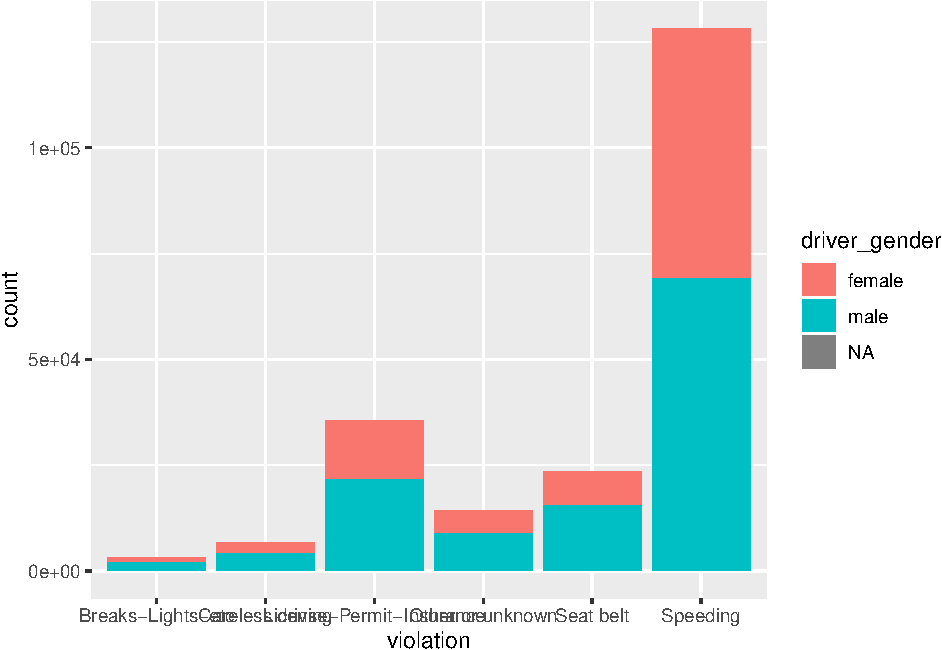
\includegraphics[width=0.7\linewidth]{R-data-viz_files/figure-latex/color-bar-gender-1}

If we wanted to see the proportions within each category we can tell
ggplot to stretch the bars between 0 and 1, we can set the position
parameter to `fill':

\begin{Shaded}
\begin{Highlighting}[]
\KeywordTok{ggplot}\NormalTok{(stops, }\KeywordTok{aes}\NormalTok{(violation)) }\OperatorTok{+}\StringTok{ }
\StringTok{  }\KeywordTok{geom_bar}\NormalTok{(}\KeywordTok{aes}\NormalTok{(}\DataTypeTok{fill =}\NormalTok{ driver_gender), }\DataTypeTok{position =} \StringTok{"fill"}\NormalTok{)}
\end{Highlighting}
\end{Shaded}

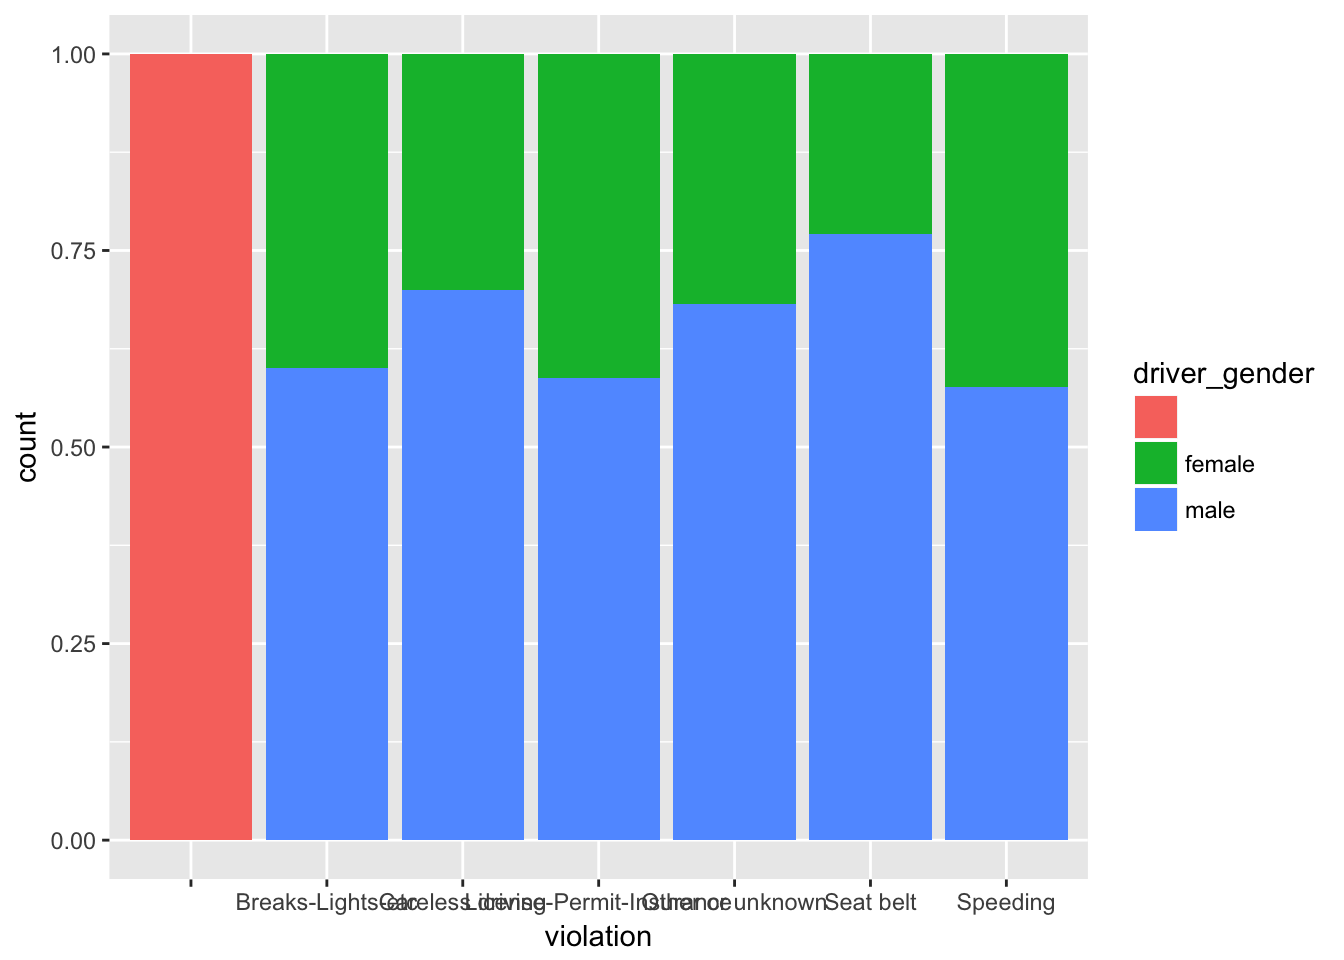
\includegraphics[width=0.7\linewidth]{R-data-viz_files/figure-latex/color-bar-stretch-1}

\begin{quote}
Challenge

Make a barplot that shows for each race the proportion of stops for male
and female drivers. How could you get rid of the NAs?
\end{quote}

To map a numerical continuous variable we use \texttt{geom\_histogram}.

\begin{quote}
Challenge

Plot a histogram that shows the distribution of drivers age. Bonus: Add
a vertical line for the mean age of the driver. Hint: there is a geom
for this!
\end{quote}

\section{Boxplot}\label{boxplot}

For this segment let's extract and work with the stops for Chickasaw
County only.

\begin{Shaded}
\begin{Highlighting}[]
\KeywordTok{library}\NormalTok{(dplyr)}
\NormalTok{Chickasaw_stops <-}\StringTok{ }\KeywordTok{filter}\NormalTok{(stops, county_name }\OperatorTok{==}\StringTok{ "Chickasaw County"}\NormalTok{)}
\end{Highlighting}
\end{Shaded}

We can use boxplots to visualize the distribution of driver age within
each violation:

\begin{Shaded}
\begin{Highlighting}[]
\KeywordTok{ggplot}\NormalTok{(}\DataTypeTok{data =}\NormalTok{ Chickasaw_stops, }\KeywordTok{aes}\NormalTok{(}\DataTypeTok{x =}\NormalTok{ violation, }\DataTypeTok{y =}\NormalTok{ driver_age)) }\OperatorTok{+}
\StringTok{    }\KeywordTok{geom_boxplot}\NormalTok{()}
\end{Highlighting}
\end{Shaded}

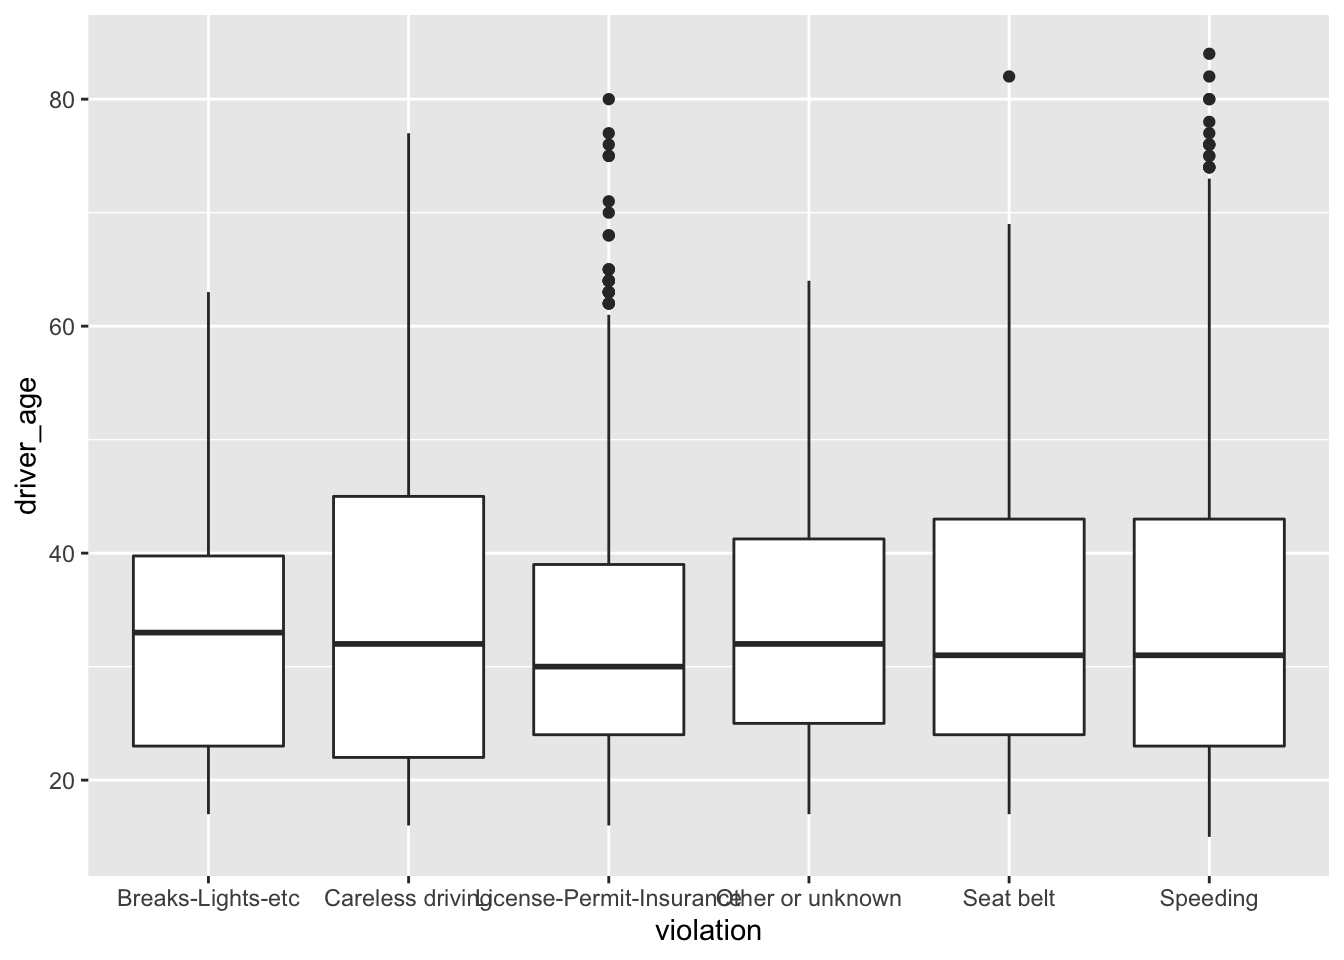
\includegraphics[width=0.7\linewidth]{R-data-viz_files/figure-latex/boxplot-1}

By adding points to boxplot, we can have a better idea of the number of
measurements and of their distribution.

\begin{Shaded}
\begin{Highlighting}[]
\KeywordTok{ggplot}\NormalTok{(}\DataTypeTok{data =}\NormalTok{ Chickasaw_stops, }\KeywordTok{aes}\NormalTok{(}\DataTypeTok{x =}\NormalTok{ violation, }\DataTypeTok{y =}\NormalTok{ driver_age)) }\OperatorTok{+}
\StringTok{    }\KeywordTok{geom_boxplot}\NormalTok{() }\OperatorTok{+}
\StringTok{    }\KeywordTok{geom_jitter}\NormalTok{()}
\end{Highlighting}
\end{Shaded}

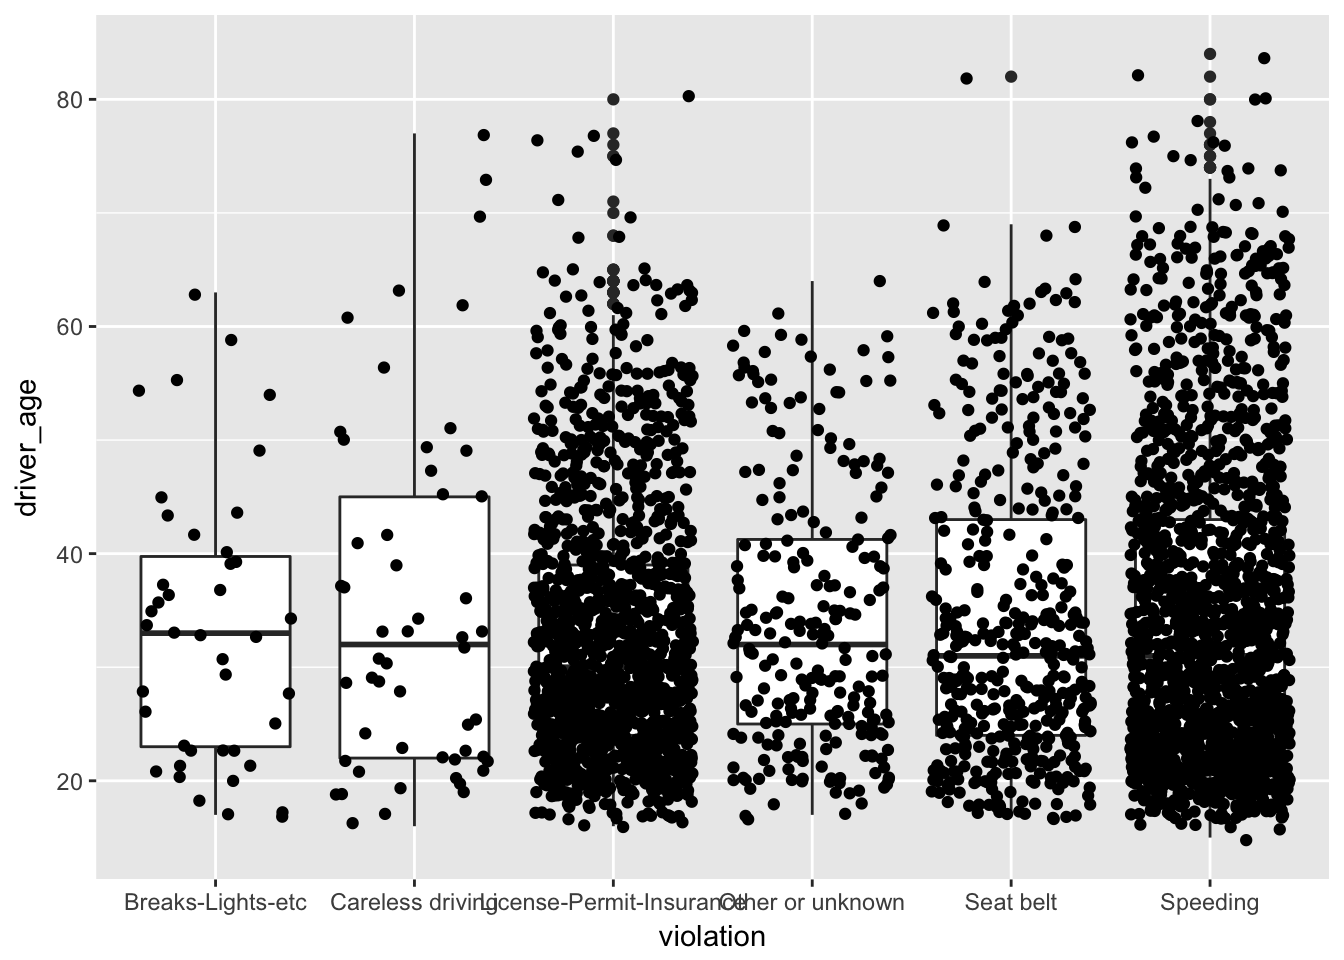
\includegraphics[width=0.7\linewidth]{R-data-viz_files/figure-latex/boxplot-with-jitter-1}

That looks quite messy. Let's clean it up by using the \texttt{alpha}
parameter to make the dots more transparent and also change their color:

\begin{Shaded}
\begin{Highlighting}[]
\KeywordTok{ggplot}\NormalTok{(}\DataTypeTok{data =}\NormalTok{ Chickasaw_stops, }\KeywordTok{aes}\NormalTok{(}\DataTypeTok{x =}\NormalTok{ violation, }\DataTypeTok{y =}\NormalTok{ driver_age)) }\OperatorTok{+}
\StringTok{    }\KeywordTok{geom_boxplot}\NormalTok{() }\OperatorTok{+}
\StringTok{    }\KeywordTok{geom_jitter}\NormalTok{(}\DataTypeTok{alpha =} \FloatTok{0.5}\NormalTok{, }\DataTypeTok{color =} \StringTok{"tomato"}\NormalTok{)}
\end{Highlighting}
\end{Shaded}

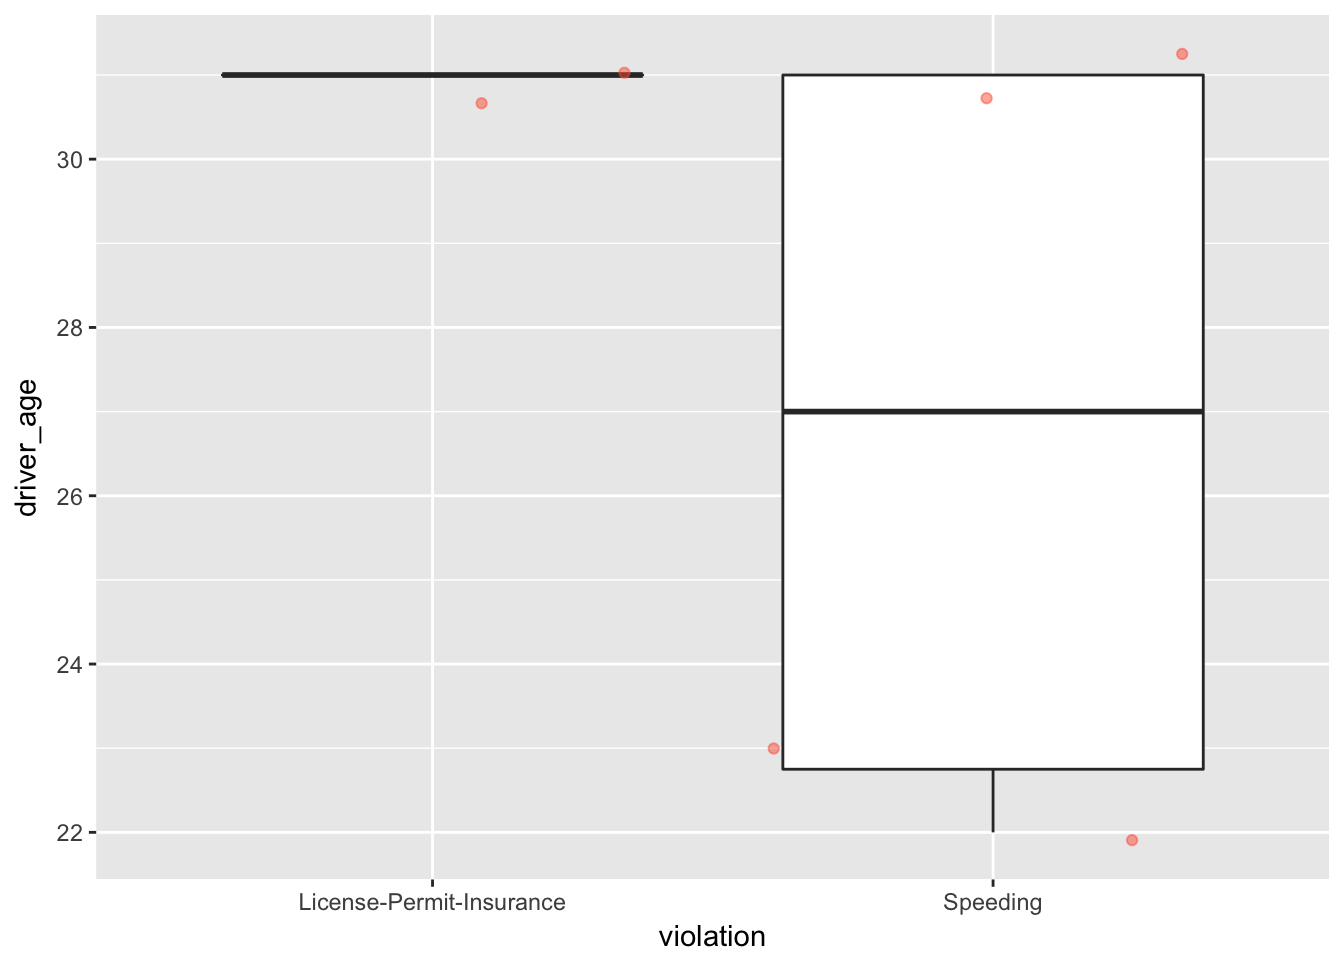
\includegraphics[width=0.7\linewidth]{R-data-viz_files/figure-latex/boxplot-with-jitter-transparent-1}

Notice how the boxplot layer is behind the jitter layer. We will change
the plotting order to keep the boxplot visible.

\begin{Shaded}
\begin{Highlighting}[]
\KeywordTok{ggplot}\NormalTok{(}\DataTypeTok{data =}\NormalTok{ Chickasaw_stops, }\KeywordTok{aes}\NormalTok{(}\DataTypeTok{x =}\NormalTok{ violation, }\DataTypeTok{y =}\NormalTok{ driver_age)) }\OperatorTok{+}
\StringTok{    }\KeywordTok{geom_jitter}\NormalTok{(}\DataTypeTok{alpha =} \FloatTok{0.1}\NormalTok{, }\DataTypeTok{color =} \StringTok{"tomato"}\NormalTok{) }\OperatorTok{+}\StringTok{ }
\StringTok{    }\KeywordTok{geom_boxplot}\NormalTok{()}
\end{Highlighting}
\end{Shaded}

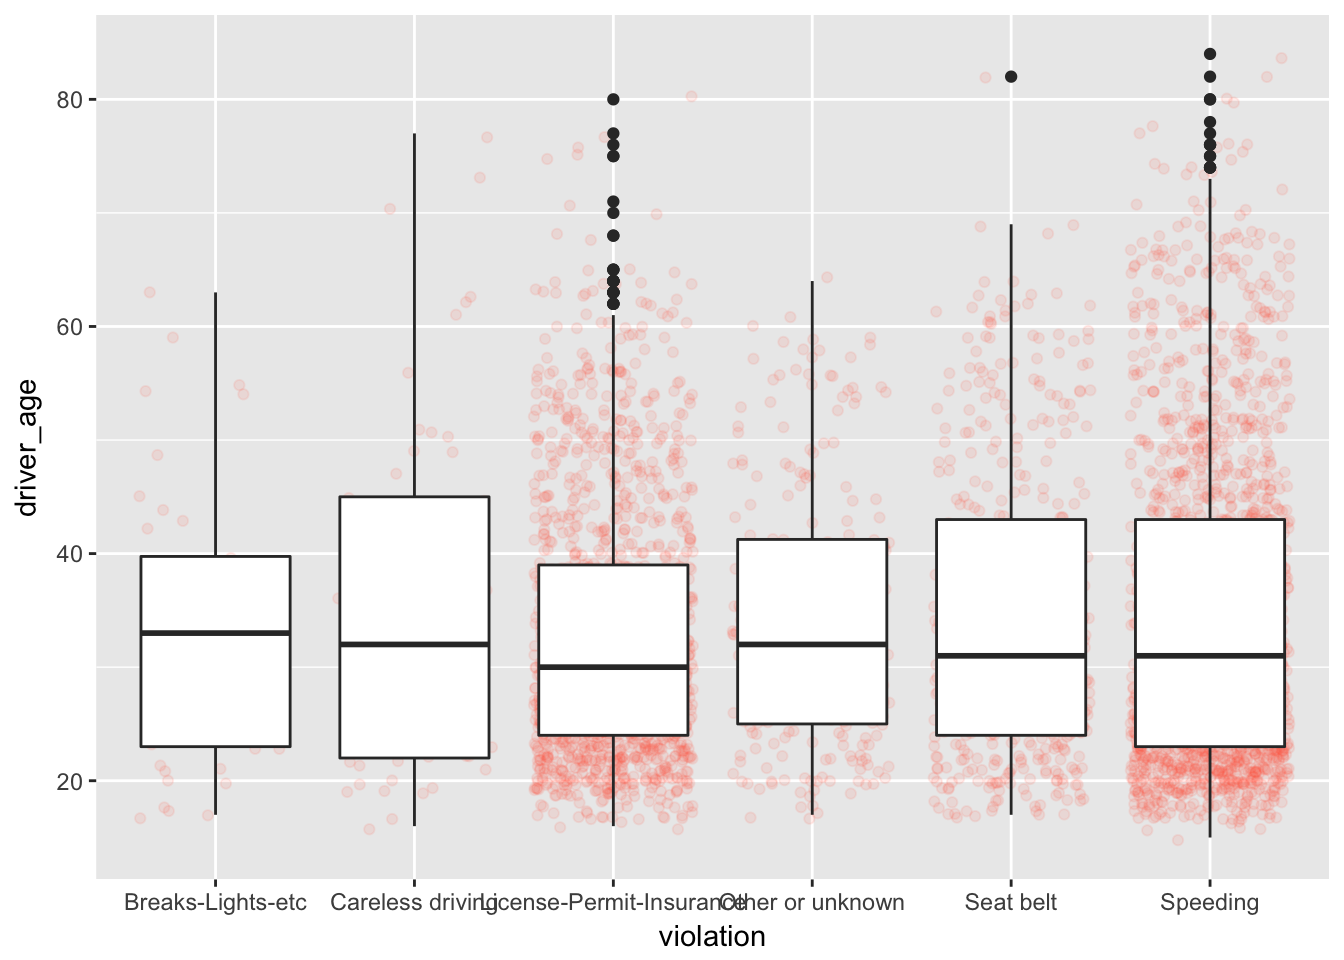
\includegraphics[width=0.7\linewidth]{R-data-viz_files/figure-latex/boxplot-with-jitter-reordered-1}

And finally we will change the transparency of the box plot so it does
not cover the points:

\begin{Shaded}
\begin{Highlighting}[]
\KeywordTok{ggplot}\NormalTok{(}\DataTypeTok{data =}\NormalTok{ Chickasaw_stops, }\KeywordTok{aes}\NormalTok{(}\DataTypeTok{x =}\NormalTok{ violation, }\DataTypeTok{y =}\NormalTok{ driver_age)) }\OperatorTok{+}
\StringTok{    }\KeywordTok{geom_jitter}\NormalTok{(}\DataTypeTok{alpha =} \FloatTok{0.1}\NormalTok{, }\DataTypeTok{color =} \StringTok{"tomato"}\NormalTok{) }\OperatorTok{+}
\StringTok{    }\KeywordTok{geom_boxplot}\NormalTok{(}\DataTypeTok{alpha =} \DecValTok{0}\NormalTok{)  }
\end{Highlighting}
\end{Shaded}

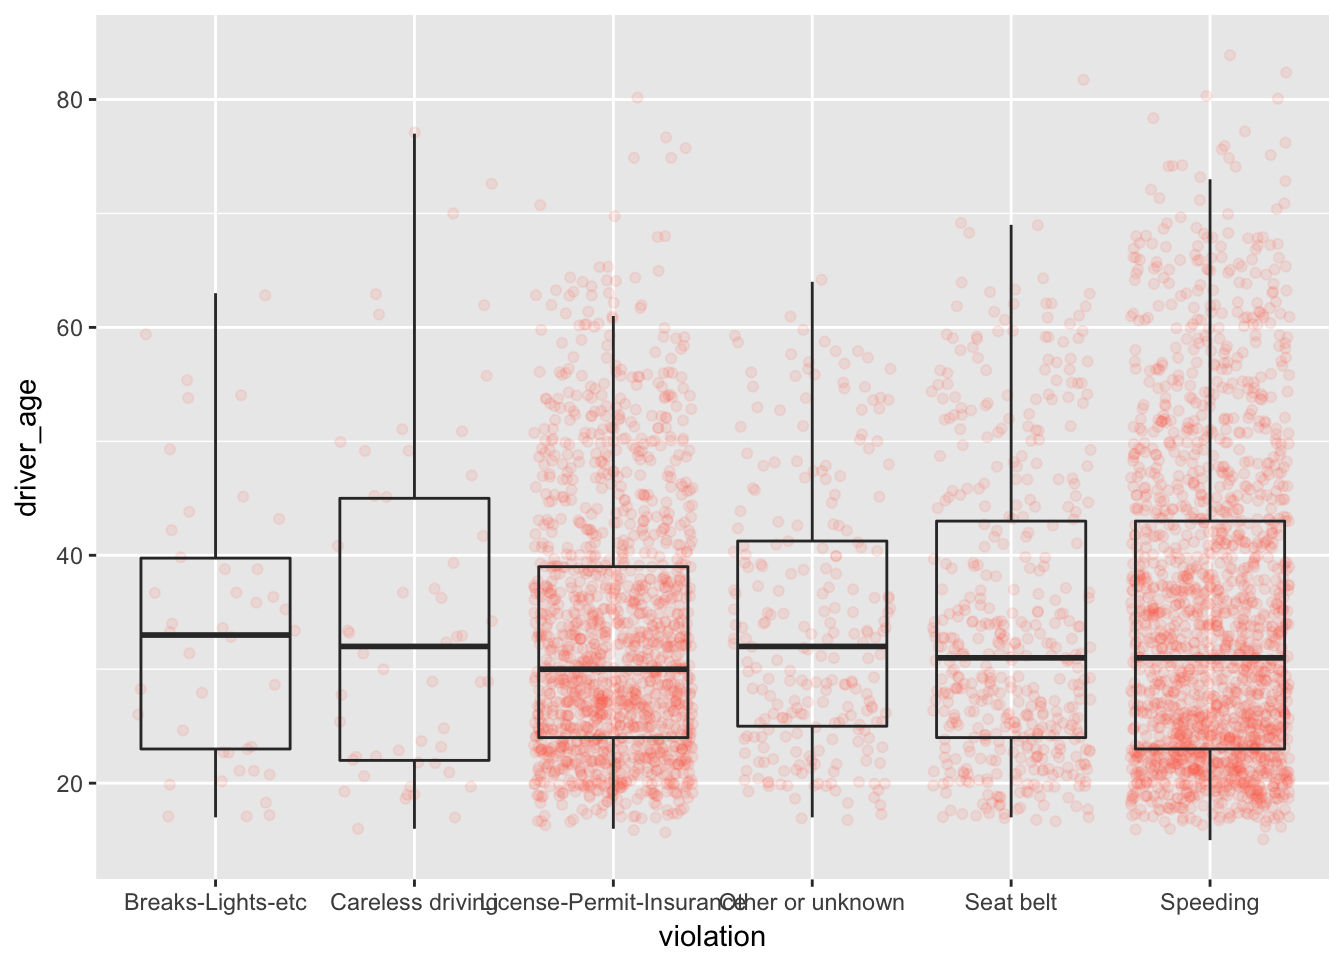
\includegraphics[width=0.7\linewidth]{R-data-viz_files/figure-latex/boxplot-with-jitter-clean-1}

Boxplots are useful summaries, but hide the \emph{shape} of the
distribution. For example, if there is a bimodal distribution, it would
not be observed with a boxplot. An alternative to the boxplot is the
violin plot (sometimes known as a beanplot), where the shape (of the
density of points) is drawn.

\begin{quote}
Challenge

\begin{itemize}
\item
  Replace the box plot of the last graph with a violin plot.
\item
  So far, we've looked at the distribution of age within violations
  Create a new plot to explore the distribution of age for another
  categorical variable.
\end{itemize}
\end{quote}

\section{Plotting time series data}\label{plotting-time-series-data}

To demonstrate time series data we will count the number of violations
for each day of the week. First we will create a table
\texttt{wd\_violations}.

\begin{Shaded}
\begin{Highlighting}[]
\NormalTok{wd_violations <-}\StringTok{ }\NormalTok{stops }\OperatorTok\StringTok{ }
\StringTok{  }\CommentTok{# group by weekday and violations:}
\StringTok{  }\KeywordTok{group_by}\NormalTok{(wk_day, violation) }\OperatorTok\StringTok{ }
\StringTok{  }\CommentTok{# count occurrences:}
\StringTok{  }\KeywordTok{tally}\NormalTok{()  }

\KeywordTok{head}\NormalTok{(wd_violations)}
\end{Highlighting}
\end{Shaded}

\begin{verbatim}
#> # A tibble: 6 x 3
#> # Groups:   wk_day [1]
#>   wk_day violation                    n
#>   <fct>  <fct>                    <int>
#> 1 Fri    Breaks-Lights-etc          564
#> 2 Fri    Careless driving          1150
#> 3 Fri    License-Permit-Insurance  6603
#> 4 Fri    Other or unknown          2603
#> 5 Fri    Seat belt                 3948
#> 6 Fri    Speeding                 20767
\end{verbatim}

Time series data can be visualized as a line plot (with -- you guessed
it! -- \texttt{geom\_line()}) mapping the days to the x axis and counts
to the y axis:

\begin{Shaded}
\begin{Highlighting}[]
\KeywordTok{ggplot}\NormalTok{(wd_violations, }\KeywordTok{aes}\NormalTok{(}\DataTypeTok{x =}\NormalTok{ wk_day, }\DataTypeTok{y =}\NormalTok{ n)) }\OperatorTok{+}
\StringTok{  }\KeywordTok{geom_line}\NormalTok{()}
\end{Highlighting}
\end{Shaded}

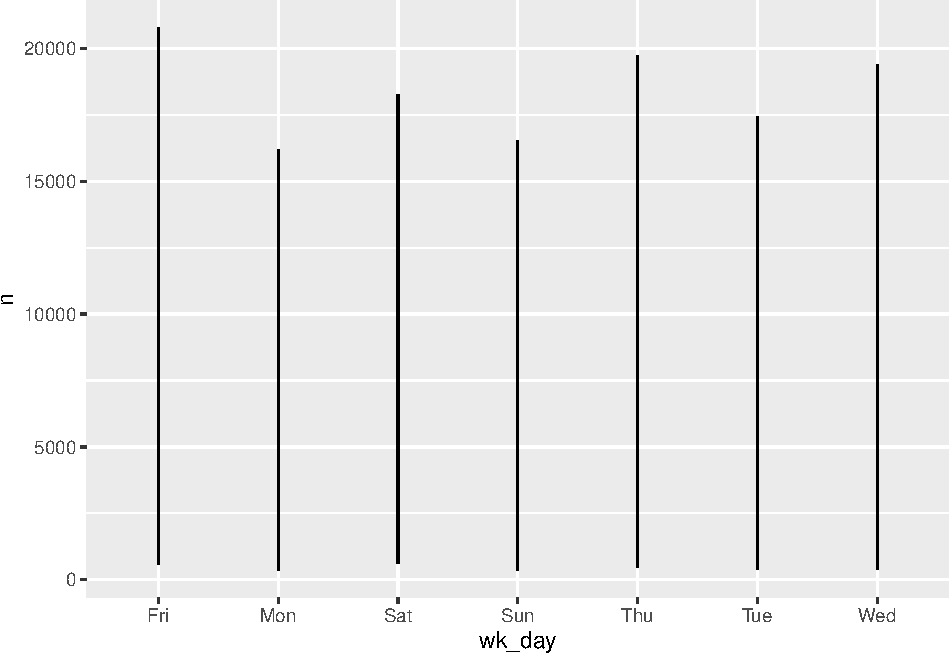
\includegraphics{R-data-viz_files/figure-latex/first-time-series-1.pdf}

Oops.

Unfortunately, there are a couple of problems with this plot.

Firstly, because we plotted data for all the violations together, ggplot
displays the \textbf{range of all values} for each day in a vertial
line. We need to tell ggplot to draw \textbf{a line for each violation}.
We do this by modifying the aesthetic function to include an instruction
to to group by violation: \texttt{group\ =\ violation}.

\begin{Shaded}
\begin{Highlighting}[]
\KeywordTok{ggplot}\NormalTok{(wd_violations, }\KeywordTok{aes}\NormalTok{(}\DataTypeTok{x =}\NormalTok{ wk_day, }\DataTypeTok{y =}\NormalTok{ n, }\DataTypeTok{group =}\NormalTok{ violation)) }\OperatorTok{+}
\StringTok{  }\KeywordTok{geom_line}\NormalTok{()}
\end{Highlighting}
\end{Shaded}

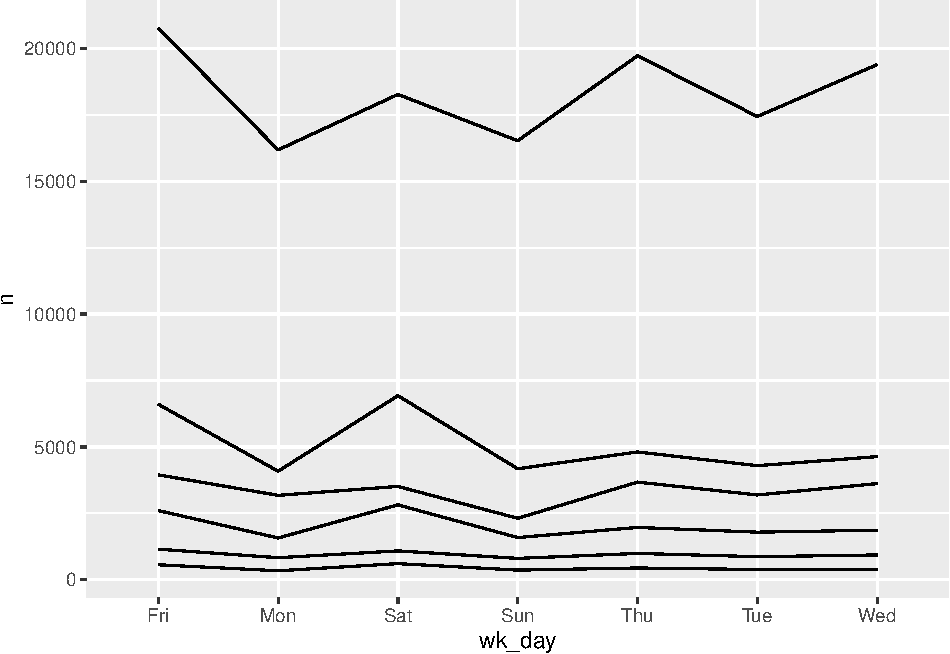
\includegraphics[width=0.7\linewidth]{R-data-viz_files/figure-latex/time-series-by-violation-1}

Secondly, the weekdays are out of order. When we read the table with
\texttt{read.csv} R determined that \texttt{wk\_day} was a factor and
assigned levels in alphabetical order.

\begin{Shaded}
\begin{Highlighting}[]
\KeywordTok{class}\NormalTok{(stops}\OperatorTok{$}\NormalTok{wk_day)}
\end{Highlighting}
\end{Shaded}

\begin{verbatim}
#> [1] "factor"
\end{verbatim}

\begin{Shaded}
\begin{Highlighting}[]
\KeywordTok{levels}\NormalTok{(stops}\OperatorTok{$}\NormalTok{wk_day)}
\end{Highlighting}
\end{Shaded}

\begin{verbatim}
#> [1] "Fri" "Mon" "Sat" "Sun" "Thu" "Tue" "Wed"
\end{verbatim}

We can reorder the levels, recreate the summary table and plot again.

\begin{Shaded}
\begin{Highlighting}[]
\NormalTok{stops}\OperatorTok{$}\NormalTok{wk_day <-}\StringTok{ }\KeywordTok{factor}\NormalTok{(stops}\OperatorTok{$}\NormalTok{wk_day, }
                       \DataTypeTok{levels=}\KeywordTok{c}\NormalTok{(}\StringTok{"Mon"}\NormalTok{, }\StringTok{"Tue"}\NormalTok{, }\StringTok{"Wed"}\NormalTok{, }\StringTok{"Thu"}\NormalTok{, }\StringTok{"Fri"}\NormalTok{, }\StringTok{"Sat"}\NormalTok{, }\StringTok{"Sun"}\NormalTok{))}

\NormalTok{wd_violations <-}\StringTok{ }\NormalTok{stops }\OperatorTok\StringTok{ }
\StringTok{  }\KeywordTok{group_by}\NormalTok{(wk_day, violation) }\OperatorTok\StringTok{ }
\StringTok{  }\KeywordTok{tally}\NormalTok{()  }

\KeywordTok{ggplot}\NormalTok{(wd_violations, }\KeywordTok{aes}\NormalTok{(}\DataTypeTok{x =}\NormalTok{ wk_day, }\DataTypeTok{y =}\NormalTok{ n, }\DataTypeTok{group =}\NormalTok{ violation)) }\OperatorTok{+}
\StringTok{  }\KeywordTok{geom_line}\NormalTok{()}
\end{Highlighting}
\end{Shaded}

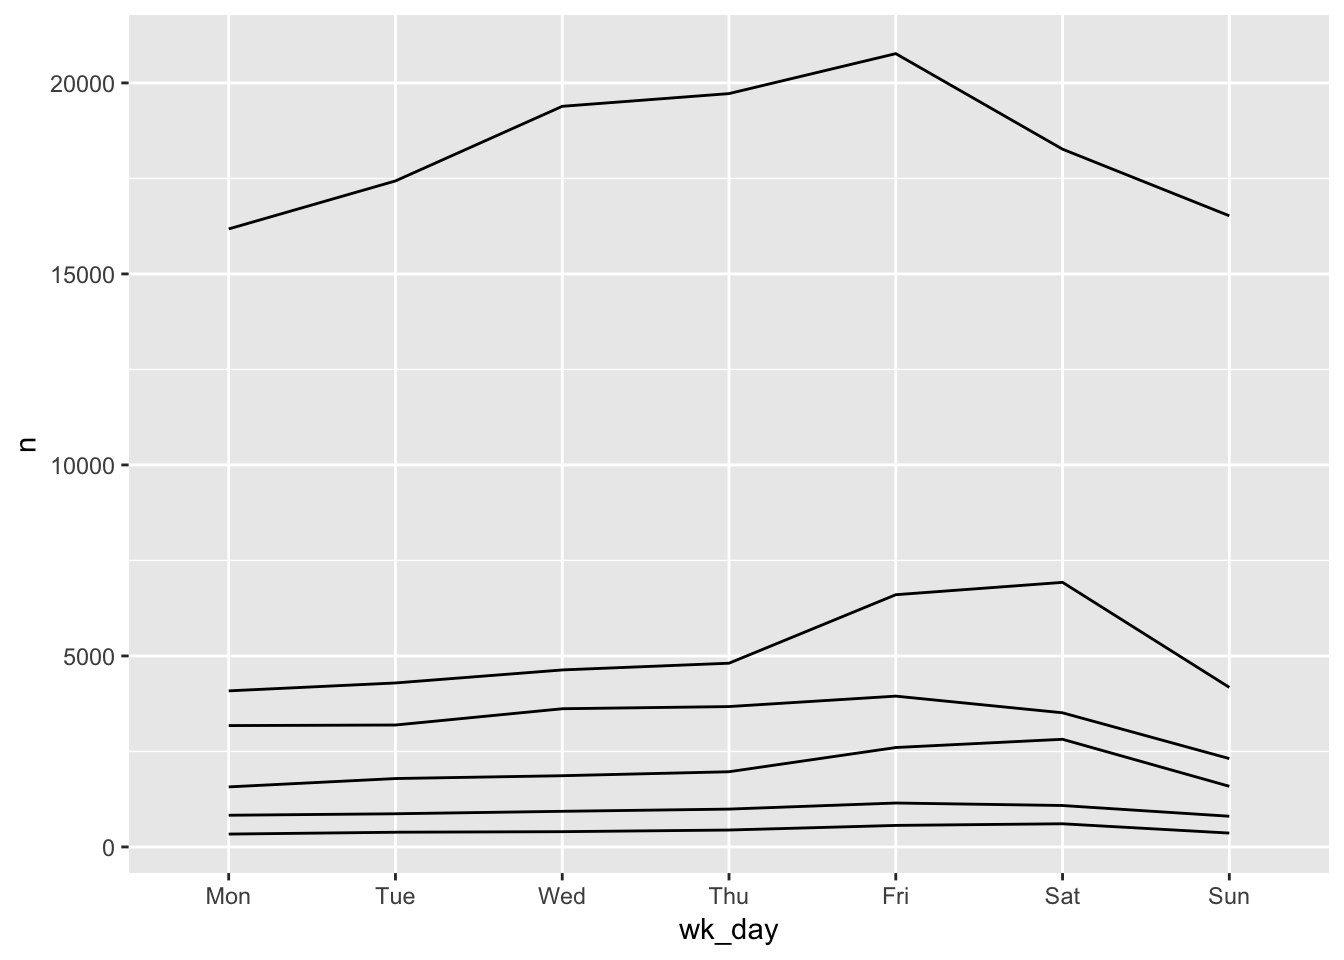
\includegraphics[width=0.7\linewidth]{R-data-viz_files/figure-latex/time-series-by-violation-order-1}

We will be able to distinguish violations in the plot if we add colors.
(If the variable is numeric \texttt{color} groups automatically.)

\begin{Shaded}
\begin{Highlighting}[]
\KeywordTok{ggplot}\NormalTok{(wd_violations, }\KeywordTok{aes}\NormalTok{(}\DataTypeTok{x =}\NormalTok{ wk_day, }\DataTypeTok{y =}\NormalTok{ n, }\DataTypeTok{group =}\NormalTok{ violation, }\DataTypeTok{color =}\NormalTok{ violation)) }\OperatorTok{+}
\StringTok{  }\KeywordTok{geom_line}\NormalTok{()}
\end{Highlighting}
\end{Shaded}

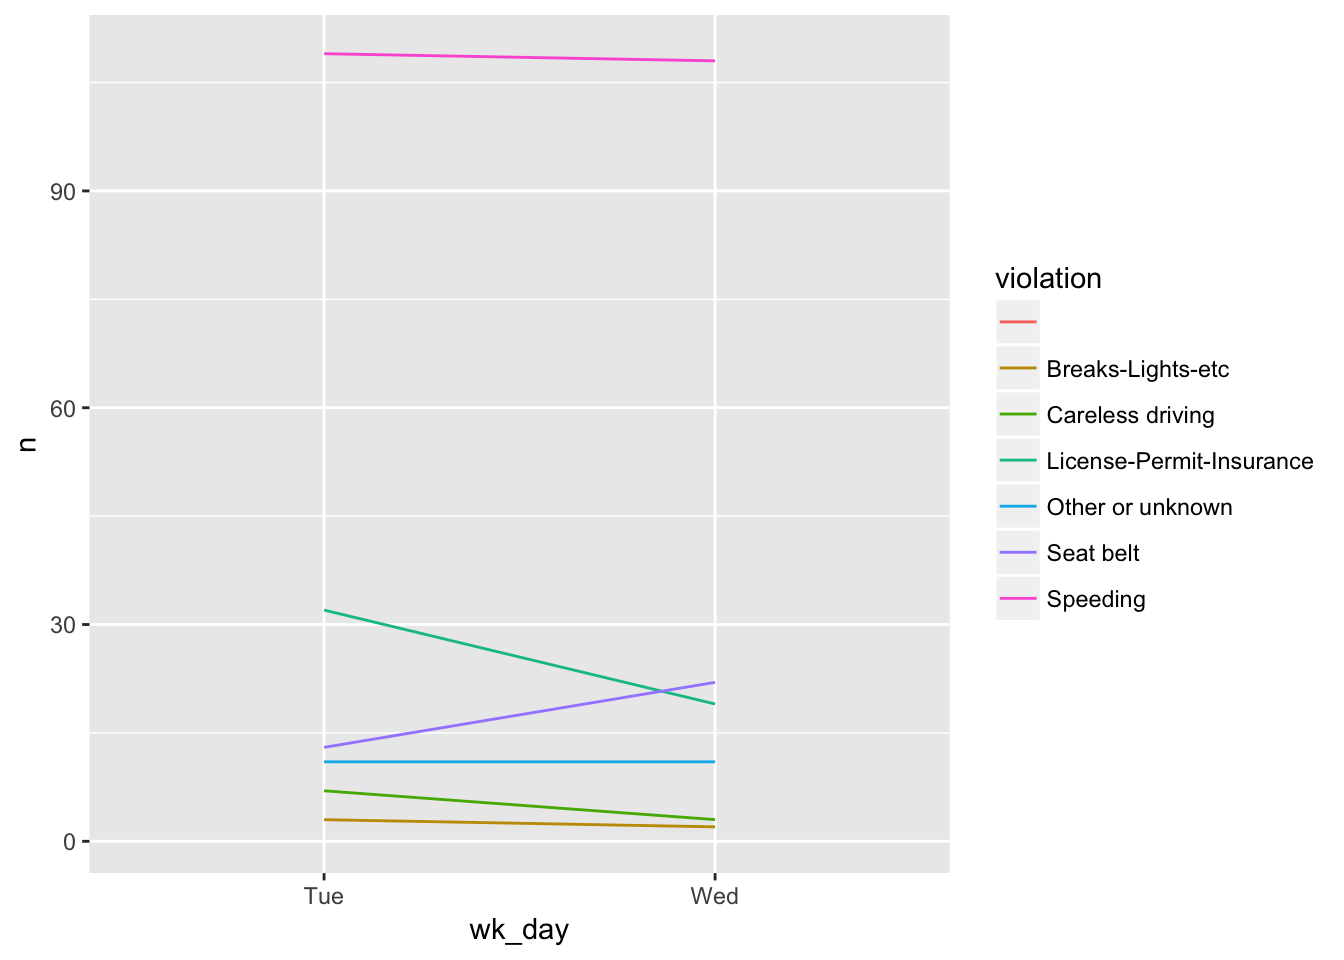
\includegraphics[width=0.7\linewidth]{R-data-viz_files/figure-latex/time-series-with-colors-1}

If you have a lot of data (like for example a
\href{https://en.wikipedia.org/wiki/Document-term_matrix}{term document
matrix}) you may want to plot your data as a heatmap. There is no
specific heatmap plotting function in ggplot2, but combining
\texttt{geom\_tile} with a smooth gradient fill
(\texttt{scale\_fill\_gradient}) does the job very well. For our weekday
example it would look like this:

\begin{Shaded}
\begin{Highlighting}[]
\KeywordTok{ggplot}\NormalTok{(wd_violations, }\KeywordTok{aes}\NormalTok{(}\DataTypeTok{x =}\NormalTok{ wk_day, }\DataTypeTok{y =}\NormalTok{ violation)) }\OperatorTok{+}
\StringTok{     }\KeywordTok{geom_tile}\NormalTok{(}\KeywordTok{aes}\NormalTok{(}\DataTypeTok{fill=}\NormalTok{n)) }\OperatorTok{+}
\StringTok{     }\KeywordTok{scale_fill_gradient}\NormalTok{(}\DataTypeTok{low=}\StringTok{"grey95"}\NormalTok{, }\DataTypeTok{high =} \StringTok{"tomato"}\NormalTok{)}
\end{Highlighting}
\end{Shaded}

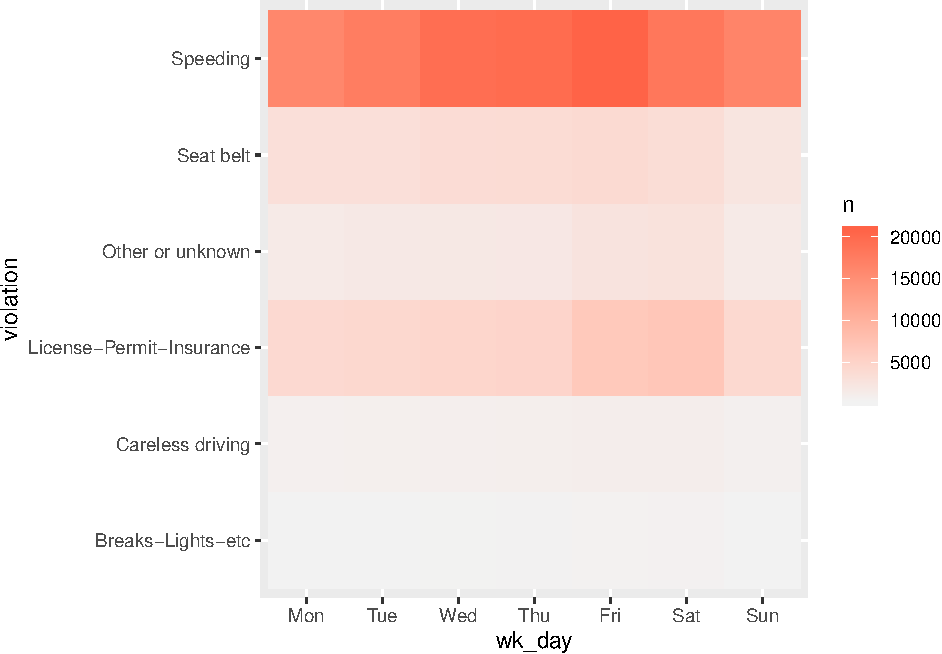
\includegraphics[width=0.7\linewidth]{R-data-viz_files/figure-latex/wdviolations-heatmap-1}

The code below show a more extensive example that maps raw violations
against day of the year.

\begin{Shaded}
\begin{Highlighting}[]
\NormalTok{stops }\OperatorTok\StringTok{ }
\StringTok{  }\KeywordTok{group_by}\NormalTok{(y_day, violation_raw) }\OperatorTok\StringTok{ }
\StringTok{  }\KeywordTok{tally}\NormalTok{() }\OperatorTok\StringTok{ }
\StringTok{  }\KeywordTok{ggplot}\NormalTok{(}\KeywordTok{aes}\NormalTok{(y_day, violation_raw)) }\OperatorTok{+}
\StringTok{     }\KeywordTok{geom_tile}\NormalTok{(}\KeywordTok{aes}\NormalTok{(}\DataTypeTok{fill=}\NormalTok{n)) }\OperatorTok{+}
\StringTok{     }\KeywordTok{scale_fill_gradient}\NormalTok{(}\DataTypeTok{low=}\StringTok{"grey95"}\NormalTok{, }\DataTypeTok{high =} \StringTok{"tomato"}\NormalTok{) }\OperatorTok{+}
\StringTok{     }\KeywordTok{theme_minimal}\NormalTok{() }\CommentTok{# (more about this below)}
\end{Highlighting}
\end{Shaded}

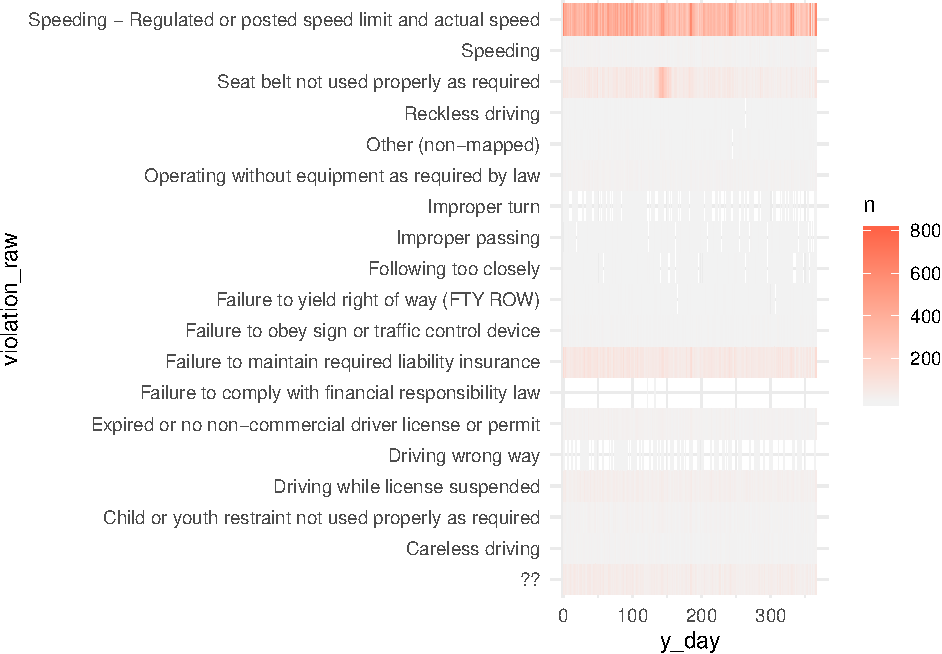
\includegraphics[width=0.7\linewidth]{R-data-viz_files/figure-latex/yday-violations-heatmap-1}

\section{Faceting}\label{faceting}

\texttt{ggplot} implements a special technique called \emph{faceting}
that allows to split one plot into multiple plots based on a factor
included in the dataset. We will use it to make a time series plot for
each violation:

\begin{Shaded}
\begin{Highlighting}[]
\KeywordTok{ggplot}\NormalTok{(wd_violations, }\KeywordTok{aes}\NormalTok{(}\DataTypeTok{x =}\NormalTok{ wk_day, }\DataTypeTok{y =}\NormalTok{ n, }\DataTypeTok{group =}\NormalTok{ violation)) }\OperatorTok{+}
\StringTok{     }\KeywordTok{geom_line}\NormalTok{() }\OperatorTok{+}
\StringTok{     }\KeywordTok{facet_wrap}\NormalTok{(}\OperatorTok{~}\StringTok{ }\NormalTok{violation)}
\end{Highlighting}
\end{Shaded}

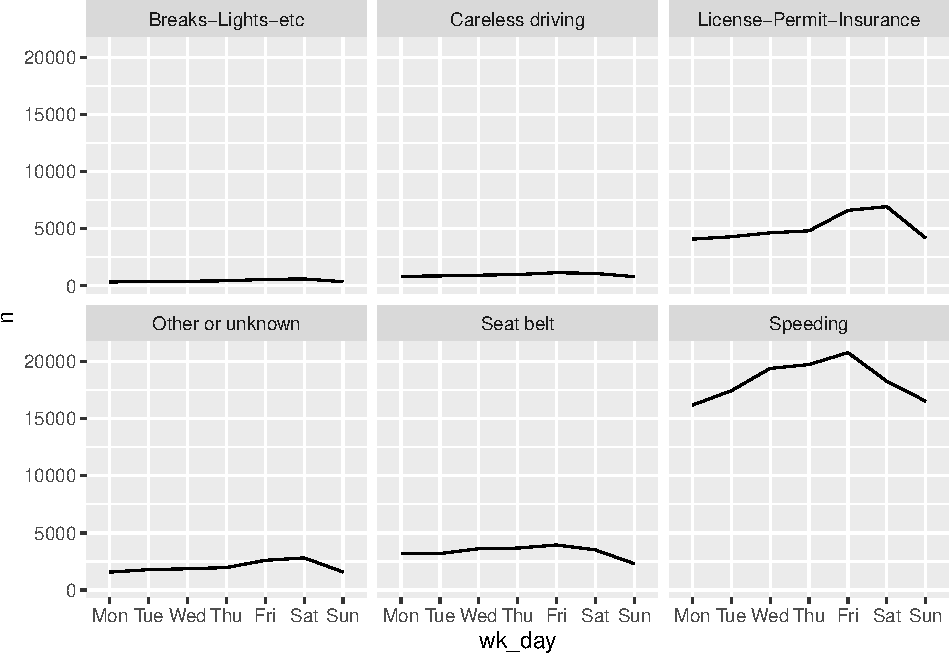
\includegraphics[width=0.7\linewidth]{R-data-viz_files/figure-latex/first-facet-1}

Now we would like to split the line in each plot by the race of the
driver. To do that we need to create a different data frame with the
counts grouped not only by \texttt{wk\_day} and \texttt{violation}, but
also \texttt{driver\_race}.

\begin{Shaded}
\begin{Highlighting}[]
\NormalTok{wd_viol_race <-}\StringTok{ }\NormalTok{stops }\OperatorTok\StringTok{ }
\StringTok{  }\KeywordTok{group_by}\NormalTok{(wk_day, violation, driver_race) }\OperatorTok
\StringTok{  }\KeywordTok{tally}\NormalTok{() }
\end{Highlighting}
\end{Shaded}

We then make the faceted plot by splitting further by race using
\texttt{color} and \texttt{group} (within a single plot):

\begin{Shaded}
\begin{Highlighting}[]
\KeywordTok{ggplot}\NormalTok{(wd_viol_race, }\KeywordTok{aes}\NormalTok{(}\DataTypeTok{x =}\NormalTok{ wk_day, }\DataTypeTok{y =}\NormalTok{ n, }\DataTypeTok{color =}\NormalTok{ driver_race, }\DataTypeTok{group =}\NormalTok{ driver_race)) }\OperatorTok{+}
\StringTok{  }\KeywordTok{geom_line}\NormalTok{() }\OperatorTok{+}\StringTok{ }
\StringTok{  }\KeywordTok{facet_wrap}\NormalTok{(}\OperatorTok{~}\StringTok{ }\NormalTok{violation)}
\end{Highlighting}
\end{Shaded}

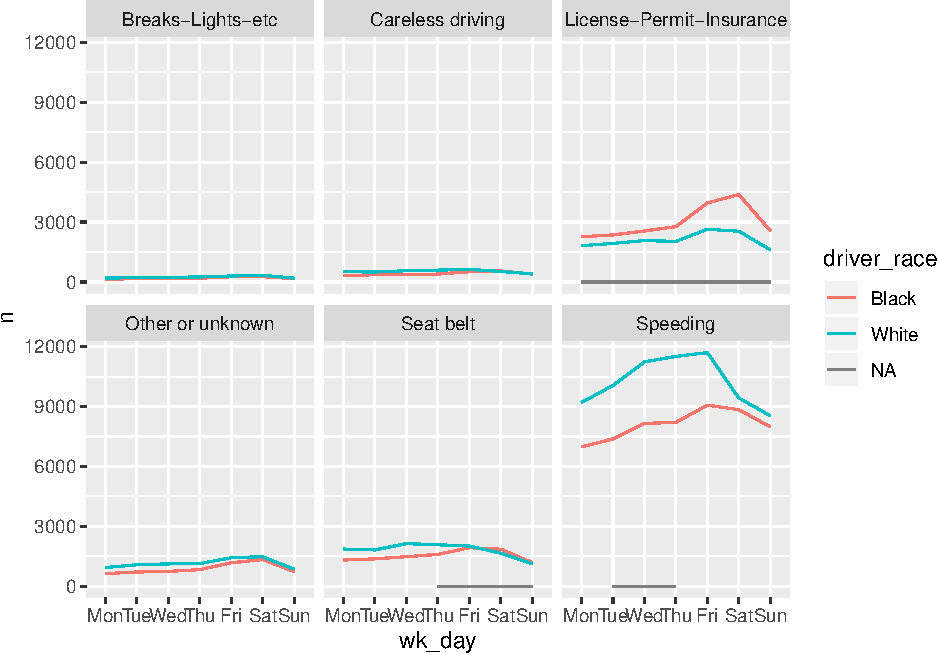
\includegraphics{R-data-viz_files/figure-latex/facet-by-violation-and-race-1.pdf}

Note that there is an alternative, the \texttt{facet\_grid} geometry,
which allows you to explicitly specify how you want your plots to be
arranged via formula notation
(\texttt{rows\ \textasciitilde{}\ columns}; a \texttt{.} can be used as
a placeholder that indicates only one row or column).

\begin{quote}
Challenge

Use what you just learned to create a plot that depicts the change of
the average age of drivers through the week for each driver race. First
create a data frame \texttt{wd\_viol\_age}, grouped by weekday, race,
and violation and calculate the mean age per grouop. Hint: Instead of
tally use \texttt{summarize(avg\_age\ =\ mean(driver\_age))} to
calculate the mean driver age. Now split your plot so we can see one
plot for each violation type. How would you go about visualizing both
lines and points on the plot?
\end{quote}

\section{\texorpdfstring{\textbf{\texttt{ggplot2}}
themes}{ggplot2 themes}}\label{ggplot2-themes}

\textbf{\texttt{ggplot2}} comes with several other themes which can be
useful to quickly change the look of your visualization, for example
\texttt{theme\_bw()} changes the plot background to white:

\begin{Shaded}
\begin{Highlighting}[]
\KeywordTok{ggplot}\NormalTok{(wd_viol_race, }\KeywordTok{aes}\NormalTok{(}\DataTypeTok{x =}\NormalTok{ wk_day, }\DataTypeTok{y =}\NormalTok{ n, }\DataTypeTok{color =}\NormalTok{ driver_race, }\DataTypeTok{group =}\NormalTok{ driver_race)) }\OperatorTok{+}
\StringTok{  }\KeywordTok{geom_line}\NormalTok{() }\OperatorTok{+}\StringTok{ }
\StringTok{  }\KeywordTok{facet_wrap}\NormalTok{(}\OperatorTok{~}\StringTok{ }\NormalTok{violation) }\OperatorTok{+}
\StringTok{  }\KeywordTok{theme_bw}\NormalTok{()}
\end{Highlighting}
\end{Shaded}

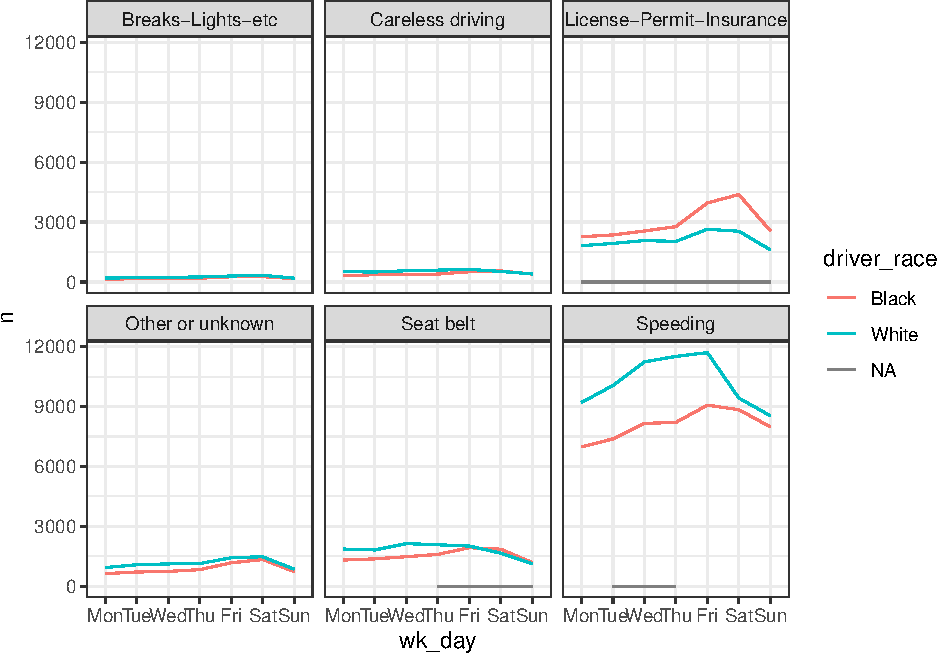
\includegraphics{R-data-viz_files/figure-latex/facet-theming-1.pdf}

The complete list of themes is available at
\url{http://docs.ggplot2.org/current/ggtheme.html}.
\texttt{theme\_minimal()} and \texttt{theme\_light()} are popular, and
\texttt{theme\_void()} can be useful as a starting point to create a new
hand-crafted theme.

The
\href{https://cran.r-project.org/web/packages/ggthemes/vignettes/ggthemes.html}{ggthemes}
package provides a wide variety of options (including an Excel 2003
theme). The
\href{http://www.ggplot2-exts.org/gallery/}{\textbf{\texttt{ggplot2}}
extensions website} provides a list of packages that extend the
capabilities of \textbf{\texttt{ggplot2}}, including additional themes.

\section{Customization}\label{customization}

There are endless possibilities to customize details of your plot,
particularly when you are ready for publication or presentation. Let's
look into just a few examples. Before we do that we will assign our plot
above to a variable.

\begin{Shaded}
\begin{Highlighting}[]
\NormalTok{stops_facet_plot <-}\StringTok{ }\KeywordTok{ggplot}\NormalTok{(wd_viol_race, }\KeywordTok{aes}\NormalTok{(}\DataTypeTok{x =}\NormalTok{ wk_day, }\DataTypeTok{y =}\NormalTok{ n, }\DataTypeTok{color =}\NormalTok{ driver_race, }\DataTypeTok{group =}\NormalTok{ driver_race)) }\OperatorTok{+}
\StringTok{  }\KeywordTok{geom_line}\NormalTok{() }\OperatorTok{+}\StringTok{ }
\StringTok{  }\KeywordTok{facet_wrap}\NormalTok{(}\OperatorTok{~}\StringTok{ }\NormalTok{violation)}
\end{Highlighting}
\end{Shaded}

Now, let's change names of axes to something more informative than
`wk\_day' and `n' and add a title to the figure:

\begin{Shaded}
\begin{Highlighting}[]
\NormalTok{stops_facet_plot }\OperatorTok{+}
\StringTok{  }\KeywordTok{labs}\NormalTok{(}\DataTypeTok{title =} \StringTok{'Observed violations per day of week'}\NormalTok{,}
         \DataTypeTok{x =} \StringTok{'Weekday of observation'}\NormalTok{,}
         \DataTypeTok{y =} \StringTok{'Number of violations'}\NormalTok{) }\OperatorTok{+}
\StringTok{  }\KeywordTok{theme_bw}\NormalTok{()}
\end{Highlighting}
\end{Shaded}

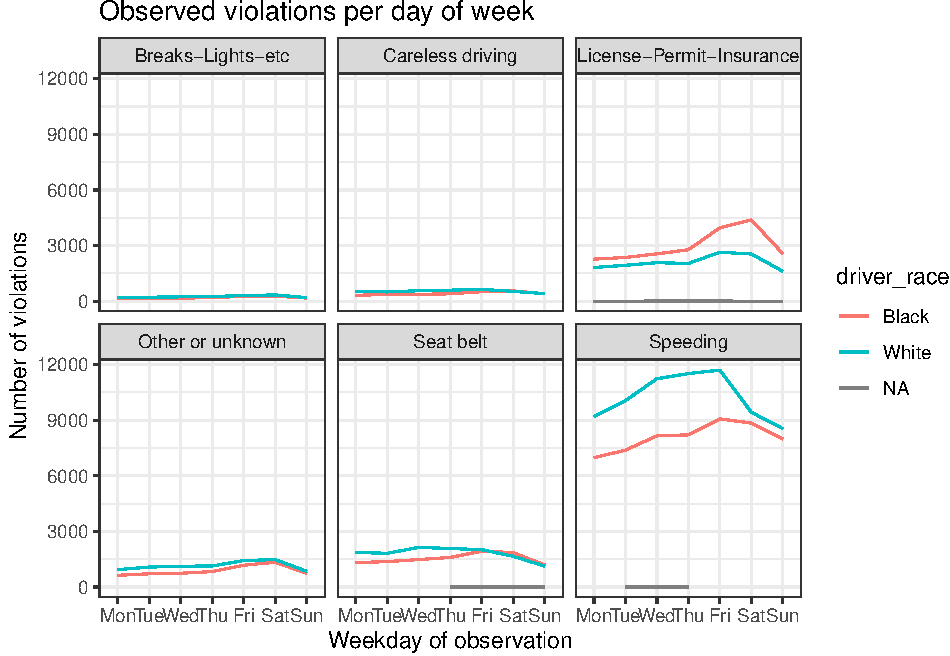
\includegraphics{R-data-viz_files/figure-latex/improved-labels-1.pdf}

The axes have more informative names, but their readability can be
improved by increasing the font size:

\begin{Shaded}
\begin{Highlighting}[]
\NormalTok{stops_facet_plot }\OperatorTok{+}
\StringTok{  }\KeywordTok{labs}\NormalTok{(}\DataTypeTok{title =} \StringTok{'Observed violations per day of week'}\NormalTok{,}
         \DataTypeTok{x =} \StringTok{'Weekday of observation'}\NormalTok{,}
         \DataTypeTok{y =} \StringTok{'Number of violations'}\NormalTok{) }\OperatorTok{+}
\StringTok{  }\KeywordTok{theme_bw}\NormalTok{() }\OperatorTok{+}\StringTok{ }
\StringTok{  }\KeywordTok{theme}\NormalTok{(}\DataTypeTok{text =} \KeywordTok{element_text}\NormalTok{(}\DataTypeTok{size=}\DecValTok{16}\NormalTok{))}
\end{Highlighting}
\end{Shaded}

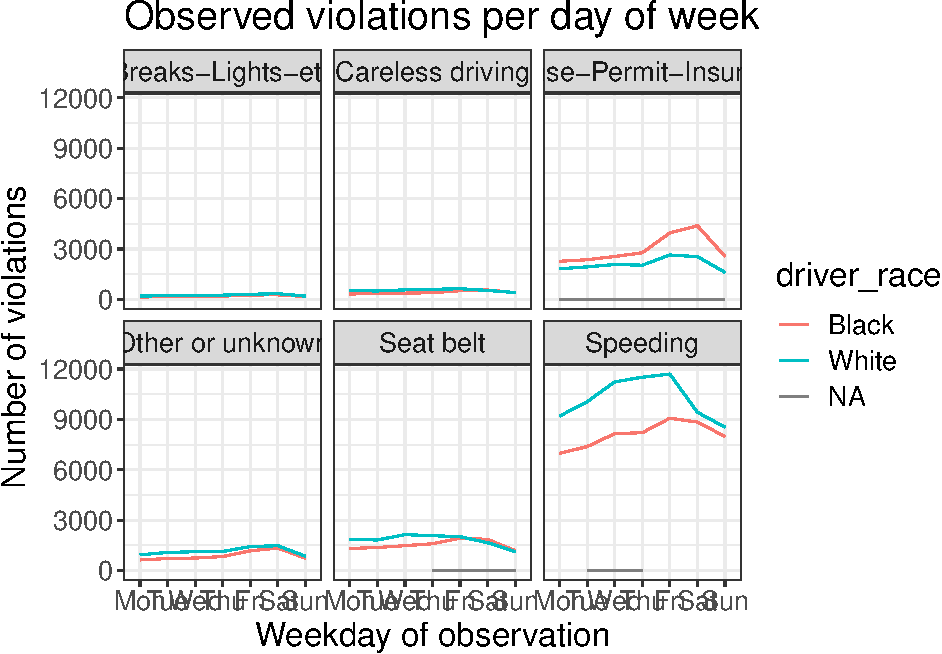
\includegraphics{R-data-viz_files/figure-latex/improved-font-size-1.pdf}

That bumps up all the text sizes, so let's manipulate them individually.

For the x-axis we will make the text smaller and adjust the labels
vertically and horizontally so they don't overlap. You can use a 90
degree angle, or experiment to find the appropriate angle for diagonally
oriented labels.

For the titles of the subplots we also reduce the size back to 12
pixels.

\begin{Shaded}
\begin{Highlighting}[]
\NormalTok{stops_facet_plot }\OperatorTok{+}
\StringTok{  }\KeywordTok{labs}\NormalTok{(}\DataTypeTok{title =} \StringTok{'Observed violations per day of week'}\NormalTok{,}
         \DataTypeTok{x =} \StringTok{'Weekday of observation'}\NormalTok{,}
         \DataTypeTok{y =} \StringTok{'Number of violations'}\NormalTok{) }\OperatorTok{+}
\StringTok{  }\KeywordTok{theme_bw}\NormalTok{() }\OperatorTok{+}\StringTok{ }
\StringTok{  }\KeywordTok{theme}\NormalTok{(}\DataTypeTok{axis.text.x =} \KeywordTok{element_text}\NormalTok{(}\DataTypeTok{colour=}\StringTok{"grey40"}\NormalTok{, }\DataTypeTok{size=}\DecValTok{12}\NormalTok{, }\DataTypeTok{angle=}\DecValTok{90}\NormalTok{, }\DataTypeTok{hjust=}\NormalTok{.}\DecValTok{5}\NormalTok{, }\DataTypeTok{vjust=}\NormalTok{.}\DecValTok{5}\NormalTok{),}
        \DataTypeTok{axis.text.y =} \KeywordTok{element_text}\NormalTok{(}\DataTypeTok{colour=}\StringTok{"grey40"}\NormalTok{, }\DataTypeTok{size=}\DecValTok{12}\NormalTok{),}
        \DataTypeTok{strip.text =} \KeywordTok{element_text}\NormalTok{(}\DataTypeTok{size=}\DecValTok{12}\NormalTok{),}
        \DataTypeTok{text =} \KeywordTok{element_text}\NormalTok{(}\DataTypeTok{size=}\DecValTok{16}\NormalTok{))}
\end{Highlighting}
\end{Shaded}

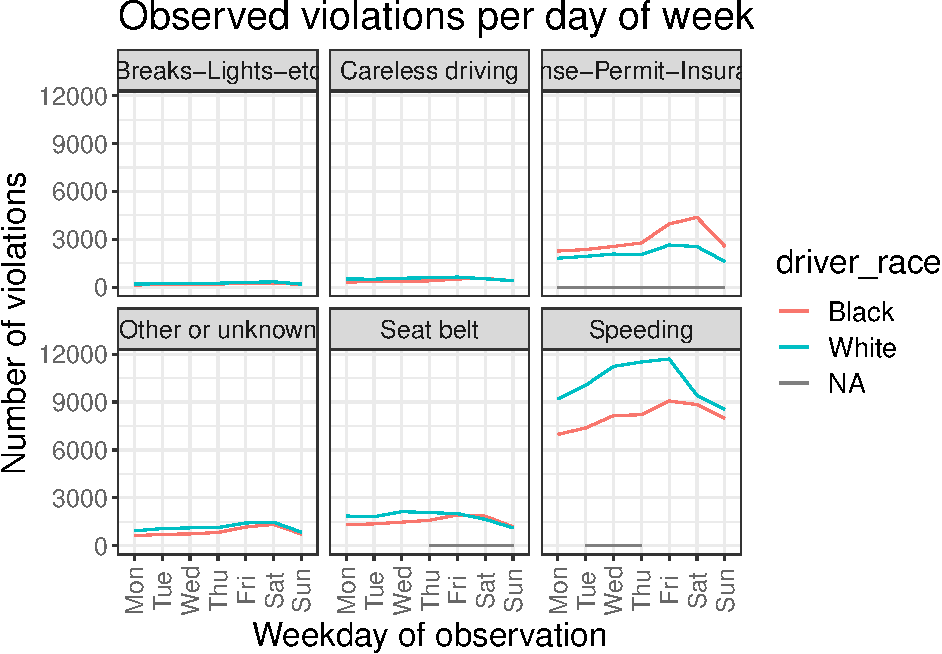
\includegraphics{R-data-viz_files/figure-latex/tilted-xlabels-1.pdf}

If you like the changes you created better than the default theme, you
can save them as an object and apply it to other plots you may create:

\begin{Shaded}
\begin{Highlighting}[]
\NormalTok{my_grey_theme <-}\StringTok{ }\KeywordTok{theme}\NormalTok{(}\DataTypeTok{axis.text.x =} \KeywordTok{element_text}\NormalTok{(}\DataTypeTok{colour=}\StringTok{"grey40"}\NormalTok{, }\DataTypeTok{size=}\DecValTok{12}\NormalTok{, }\DataTypeTok{angle=}\DecValTok{90}\NormalTok{, }\DataTypeTok{hjust=}\NormalTok{.}\DecValTok{5}\NormalTok{, }\DataTypeTok{vjust=}\NormalTok{.}\DecValTok{5}\NormalTok{),}
                   \DataTypeTok{axis.text.y =} \KeywordTok{element_text}\NormalTok{(}\DataTypeTok{colour=}\StringTok{"grey40"}\NormalTok{, }\DataTypeTok{size=}\DecValTok{12}\NormalTok{), }\DataTypeTok{text=}\KeywordTok{element_text}\NormalTok{(}\DataTypeTok{size=}\DecValTok{16}\NormalTok{))}

\KeywordTok{ggplot}\NormalTok{(}\DataTypeTok{data =}\NormalTok{ Chickasaw_stops, }\KeywordTok{aes}\NormalTok{(}\DataTypeTok{x =}\NormalTok{ violation, }\DataTypeTok{y =}\NormalTok{ driver_age)) }\OperatorTok{+}
\StringTok{  }\KeywordTok{geom_boxplot}\NormalTok{() }\OperatorTok{+}\StringTok{ }
\StringTok{  }\NormalTok{my_grey_theme}
\end{Highlighting}
\end{Shaded}

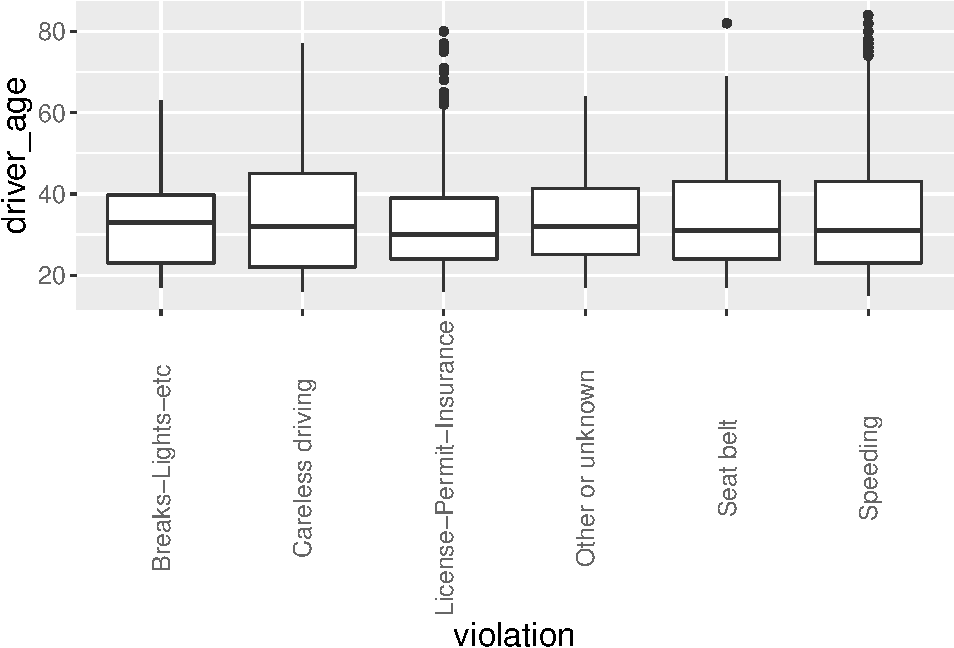
\includegraphics{R-data-viz_files/figure-latex/save-reapply-theme-1.pdf}

Note that it is also possible to change the fonts of your plots. If you
are on Windows, you may have to install the
\href{https://github.com/wch/extrafont}{\textbf{extrafont} package}, and
follow the instructions included in the README for this package.

After creating your plot, you can save it out to a file in your prefered
format. You can change the dimension (and resolution) of your plot by
adjusting the appropriate arguments (\texttt{width}, \texttt{height} and
\texttt{dpi}):

\begin{Shaded}
\begin{Highlighting}[]
\NormalTok{my_plot <-}\StringTok{ }\NormalTok{stops_facet_plot }\OperatorTok{+}
\StringTok{  }\KeywordTok{labs}\NormalTok{(}\DataTypeTok{title =} \StringTok{'Observed violations per day of week'}\NormalTok{,}
         \DataTypeTok{x =} \StringTok{'Weekday of observation'}\NormalTok{,}
         \DataTypeTok{y =} \StringTok{'Number of violations'}\NormalTok{) }\OperatorTok{+}
\StringTok{  }\KeywordTok{theme_bw}\NormalTok{() }\OperatorTok{+}\StringTok{ }
\StringTok{  }\KeywordTok{theme}\NormalTok{(}\DataTypeTok{axis.text.x =} \KeywordTok{element_text}\NormalTok{(}\DataTypeTok{colour=}\StringTok{"grey40"}\NormalTok{, }\DataTypeTok{size=}\DecValTok{12}\NormalTok{, }\DataTypeTok{angle=}\DecValTok{90}\NormalTok{, }\DataTypeTok{hjust=}\NormalTok{.}\DecValTok{5}\NormalTok{, }\DataTypeTok{vjust=}\NormalTok{.}\DecValTok{5}\NormalTok{),}
        \DataTypeTok{axis.text.y =} \KeywordTok{element_text}\NormalTok{(}\DataTypeTok{colour=}\StringTok{"grey40"}\NormalTok{, }\DataTypeTok{size=}\DecValTok{12}\NormalTok{),}
        \DataTypeTok{strip.text =} \KeywordTok{element_text}\NormalTok{(}\DataTypeTok{size=}\DecValTok{14}\NormalTok{),}
        \DataTypeTok{text =} \KeywordTok{element_text}\NormalTok{(}\DataTypeTok{size=}\DecValTok{16}\NormalTok{))}

\KeywordTok{ggsave}\NormalTok{(}\StringTok{"name_of_file.png"}\NormalTok{, my_plot, }\DataTypeTok{width=}\DecValTok{15}\NormalTok{, }\DataTypeTok{height=}\DecValTok{10}\NormalTok{)}
\end{Highlighting}
\end{Shaded}

Note: The parameters \texttt{width} and \texttt{height} also determine
the font size in the saved plot.

\begin{quote}
Challenge

Improve one of the plots you generated or create a beautiful graph of
your own and save it to your desktop. Use the RStudio
\href{https://www.rstudio.com/wp-content/uploads/2016/11/ggplot2-cheatsheet-2.1.pdf}{\textbf{\texttt{ggplot2}}
cheat sheet} for inspiration.

Here are some ideas: * See if you can change the thickness of the lines.
* Can you find a way to change the name of the legend? What about its
labels? * Try using a different color palette (see
\url{http://www.cookbook-r.com/Graphs/Colors_(ggplot2)/}).
\end{quote}

\chapter{Interactive graphs}\label{interactive-graphs}

\begin{quote}
Learning Objectives

\begin{itemize}
\tightlist
\item
  Be aware of R interactive graphing capabilities and options
\item
  Know some graphing packages that are based on htmlwidgets
\item
  Create a simple interactive plot
\item
  Understand the basic structure of a \texttt{shiny} app
\end{itemize}
\end{quote}

\begin{center}\rule{0.5\linewidth}{\linethickness}\end{center}

\section{\texorpdfstring{\textbf{\texttt{htmlwidgets}}}{htmlwidgets}}\label{htmlwidgets}

JavaScript is probably the most widely used scripting languages to
create interactive webpages (html). The
\href{(https://CRAN.R-project.org/package=htmlwidgets)}{\texttt{htmlwidgets}
package} provides a framework to bind R commands to various existing,
interactive JavaScript libraries, including those that greate data
graphs. The interactive components (``widgets'') created using the
framework can be:

\begin{itemize}
\tightlist
\item
  used at the R console for data analysis just like conventional R plots
  (via RStudio Viewer).
\item
  seamlessly embedded within R Markdown documents and Shiny web
  applications.
\item
  saved as standalone web pages for ad-hoc sharing via email, Dropbox,
  etc.
\end{itemize}

While you can certainly develop yor own widget, there are a number of
widgets already available, that you can install and that make creating
interacive visualizations much easier. In fact, the packages used for
the examples in section \ref{domain} are all based on htmlwidgets.

For a complete list check out the
\href{http://gallery.htmlwidgets.org}{htmlwidgets gallery}.

The \texttt{htmlwidgets} framework ensures that the graphics are
rendered locally. By default they either run in your web browser or in
the R Studio viewer. If you use \href{https://rmarkdown.rstudio.com/}{R
Markdown}, the html pages rendered contain the full JavaScript code, so
you can also also deploy them to a standard webserver (like github
pages).

\section{\texorpdfstring{\textbf{\texttt{plotly}}}{plotly}}\label{plotly}

We will start with a widget called \texttt{plotly}. \texttt{plotly}
binds R commands to the \href{https://plot.ly/javascript/}{JavaScript
plotly.js graphing library}. The R package allows you to easily
translate \texttt{ggplot2} graphics to an interactive web-based version.

First we install and load the package.

\begin{Shaded}
\begin{Highlighting}[]
\KeywordTok{install.packages}\NormalTok{(plotly) }\CommentTok{# if you haven't installed the package}
\KeywordTok{library}\NormalTok{(plotly)}
\end{Highlighting}
\end{Shaded}

Let us go back to our initial scatterplot.

\begin{Shaded}
\begin{Highlighting}[]
\KeywordTok{ggplot}\NormalTok{(}\DataTypeTok{data =}\NormalTok{ stops_county, }\KeywordTok{aes}\NormalTok{(}\DataTypeTok{x =}\NormalTok{ pct_black_stopped, }\DataTypeTok{y =}\NormalTok{ pct_white_stopped)) }\OperatorTok{+}
\StringTok{  }\KeywordTok{geom_point}\NormalTok{()}
\end{Highlighting}
\end{Shaded}

To turn this into an interactive graph with \texttt{plotly}, we create a
ggplot object by assigning it to a variable:

\begin{Shaded}
\begin{Highlighting}[]
\NormalTok{p <-}\StringTok{ }\KeywordTok{ggplot}\NormalTok{(}\DataTypeTok{data =}\NormalTok{ stops_county, }\KeywordTok{aes}\NormalTok{(}\DataTypeTok{x =}\NormalTok{ pct_black_stopped, }\DataTypeTok{y =}\NormalTok{ pct_white_stopped)) }\OperatorTok{+}
\StringTok{  }\KeywordTok{geom_point}\NormalTok{()}
\end{Highlighting}
\end{Shaded}

We can then pass that object to the \texttt{ggplotly} function (the dev.
version of ggplot2 has a \texttt{ggplotly()} function, but this works):

\begin{Shaded}
\begin{Highlighting}[]
\KeywordTok{ggplotly}\NormalTok{(p) }
\end{Highlighting}
\end{Shaded}

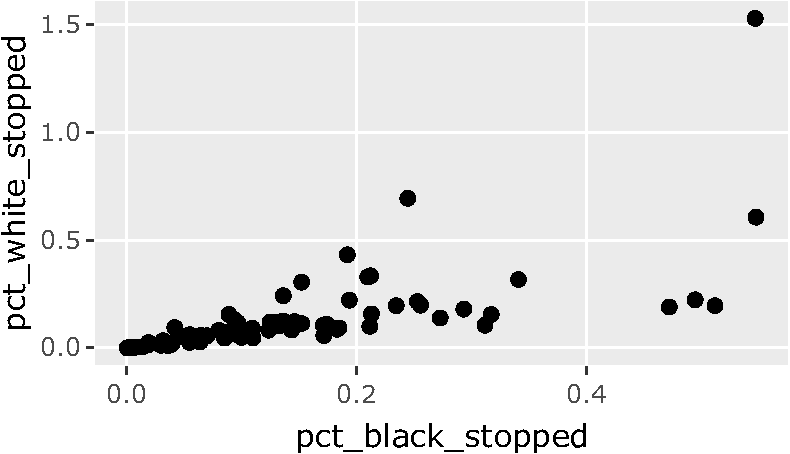
\includegraphics{R-data-viz_files/figure-latex/ggplotly-scatter-1.pdf}

This is really all that is to it.

ALternatively, it is possible to forgo ggplot and using the
\texttt{plot\_ly} function to create your graph from scratch. For our
example that would be:

\begin{Shaded}
\begin{Highlighting}[]
\KeywordTok{plot_ly}\NormalTok{(stops_county, }\DataTypeTok{x =} \OperatorTok{~}\NormalTok{pct_black_stopped, }\DataTypeTok{y =} \OperatorTok{~}\NormalTok{pct_white_stopped)}
\end{Highlighting}
\end{Shaded}

\begin{verbatim}
#> No trace type specified:
#>   Based on info supplied, a 'scatter' trace seems appropriate.
#>   Read more about this trace type -> https://plot.ly/r/reference/#scatter
\end{verbatim}

\begin{verbatim}
#> No scatter mode specifed:
#>   Setting the mode to markers
#>   Read more about this attribute -> https://plot.ly/r/reference/#scatter-mode
\end{verbatim}

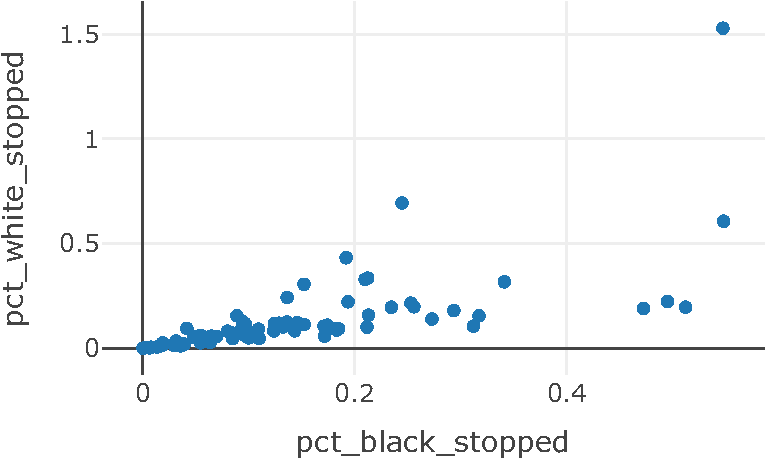
\includegraphics{R-data-viz_files/figure-latex/plotly-scatter-1.pdf}

\begin{quote}
Challenge

Go back to the box plot we created earlier using the Chickasaw\_stops:
\texttt{ggplot(Chickasaw\_stops,\ aes(x\ =\ violation,\ y\ =\ driver\_age))\ +}
\texttt{geom\_boxplot()} Create an interactive version of it, using both
approaches, \texttt{ggplotly} and \texttt{plot\_ly}.
\end{quote}

The full documentation of all the arguments \texttt{plot\_ly} can take
is here: \url{https://plot.ly/r/reference/}

\section{shiny}\label{shiny}

\texttt{htmlwidgets} are very powerful, but if you require more
customization and flexibility, particularly with regard to user input,
you may want to look into
\href{https://CRAN.R-project.org/package=shiny}{\texttt{shiny}}. Because
it executes acutal R code, which web browsers cannot execute,
\texttt{shiny} requires its own server.

There are verious ways in which a shiny application can be run. We will
use an example run it from the

R Commandline.

Rmarkdown: To call Shiny code from an R Markdown document, add runtime:
shiny to the header shiny server: either run your own, or host it at
ShinyApps.io

Building shiny apps deserves its own workshop, so here - to give you a
teaser - I have provided only a very simple example. We will re-use our
barchart from earlier where we plotted the proportional amount of
traffic violations for each gender:

\begin{Shaded}
\begin{Highlighting}[]
\KeywordTok{ggplot}\NormalTok{(stops, }\KeywordTok{aes}\NormalTok{(violation)) }\OperatorTok{+}\StringTok{ }
\StringTok{        }\KeywordTok{geom_bar}\NormalTok{(}\KeywordTok{aes}\NormalTok{(}\DataTypeTok{fill =}\NormalTok{ driver_gender), }\DataTypeTok{position =} \StringTok{"fill"}\NormalTok{)}
\end{Highlighting}
\end{Shaded}

We want to create a plot where we can choose which county we'd like to
display this bar chart for.

I have prepared the code for this, which you can run like this:

\begin{enumerate}
\def\labelenumi{\arabic{enumi}.}
\item
  Install and load the \texttt{shiny} package
  (\texttt{install.packages(shiny)}).
\item
  In your \texttt{R-data-viz} folder create a new folder called
  \texttt{shinyapps}.
\item
  Download \texttt{app.R} into that folder:
\end{enumerate}

\begin{Shaded}
\begin{Highlighting}[]
\KeywordTok{download.file}\NormalTok{(}\StringTok{"https://raw.githubusercontent.com/cengel/R-data-viz/master/shinyapp/app.R"}\NormalTok{, }\StringTok{"shinyapp/app.R"}\NormalTok{)}
\end{Highlighting}
\end{Shaded}

\begin{enumerate}
\def\labelenumi{\arabic{enumi}.}
\setcounter{enumi}{3}
\tightlist
\item
  In your R console:
\end{enumerate}

\begin{Shaded}
\begin{Highlighting}[]
\KeywordTok{library}\NormalTok{(shiny)}
\KeywordTok{runApp}\NormalTok{(}\StringTok{"./shinyapp/"}\NormalTok{)}
\end{Highlighting}
\end{Shaded}

Let us now go over the code in the \texttt{app.R} script.

We define two functions and call them \texttt{ui} (for user interface,
which we present to the user and receive input) and \texttt{server}
(where the input is used and the magic happens).

This is what happens in the \texttt{ui} function:

Using some of the layout functions shiny comes with we define a panel
with a sidebar, where the input is received the main panel, where the
plot is going to be displahyed. We also assign the plot a name
(\texttt{violationsPlot}) that we will reuse later. Lastly we add some
text to help users understand what this graph about.

A very important function is \texttt{selectInput}, where we define the
choices that the user has (the county names in the table) and also
define the name of the variable that will hold the input from the user:
\texttt{county}.

The \texttt{server} is where input and output are processed. In this
example we really only render the plot. You see that the name for our
plot (\texttt{violationsPlot}) appears attached to the \texttt{output}
variable. You can also detect our ggplot code from earlier, with the
only difference that we use the input county value
\texttt{input\$county} to filter the data frame before we send them to
ggplot to plot.

The very last line of the script binds the two together as a shiny app.

\begin{Shaded}
\begin{Highlighting}[]
\KeywordTok{library}\NormalTok{(shiny)}
\KeywordTok{library}\NormalTok{(ggplot2)}
\KeywordTok{library}\NormalTok{(dplyr)}

\CommentTok{# uncomment this if you need to reload the stops table}
\CommentTok{# stops <- read.csv('https://github.com/cengel/R-data-viz/raw/master/data/MS_stops.csv')}

\NormalTok{## UI}
\CommentTok{# Use a fluid Bootstrap layout}
\NormalTok{ui <-}\StringTok{ }\KeywordTok{fluidPage}\NormalTok{(    }
  
  \CommentTok{# Give the page a title}
  \KeywordTok{titlePanel}\NormalTok{(}\StringTok{"Missisippi Violations by County"}\NormalTok{),}
  
  \CommentTok{# Generate a row with a sidebar}
  \KeywordTok{sidebarLayout}\NormalTok{(      }
    
    \CommentTok{# Define the sidebar with one input}
    \KeywordTok{sidebarPanel}\NormalTok{(}
      \KeywordTok{selectInput}\NormalTok{(}\StringTok{"county"}\NormalTok{, }\StringTok{"County:"}\NormalTok{, }
                  \DataTypeTok{choices=}\KeywordTok{unique}\NormalTok{(stops}\OperatorTok{$}\NormalTok{county_name)),}
      \KeywordTok{hr}\NormalTok{(),}
      \KeywordTok{helpText}\NormalTok{(}\StringTok{"Data from Stanford Openpolicing Project."}\NormalTok{)}
\NormalTok{    ),}
    
    \CommentTok{# Create a spot for the barplot}
    \KeywordTok{mainPanel}\NormalTok{(}
      \KeywordTok{plotOutput}\NormalTok{(}\StringTok{"violationsPlot"}\NormalTok{)  }
\NormalTok{    )}
    
\NormalTok{  )}
\NormalTok{)}

\NormalTok{## Server}

\CommentTok{# Define a server for the Shiny app}
\NormalTok{server <-}\StringTok{ }\ControlFlowTok{function}\NormalTok{(input, output) \{}
  
  \CommentTok{# Fill in the spot we created for a plot}
\NormalTok{  output}\OperatorTok{$}\NormalTok{violationsPlot <-}\StringTok{ }\KeywordTok{renderPlot}\NormalTok{(\{}
    
\NormalTok{    stops }\OperatorTok\StringTok{ }
\StringTok{      }\KeywordTok{filter}\NormalTok{(county_name }\OperatorTok{==}\StringTok{ }\NormalTok{input}\OperatorTok{$}\NormalTok{county) }\OperatorTok\StringTok{ }
\StringTok{      }\KeywordTok{ggplot}\NormalTok{(}\KeywordTok{aes}\NormalTok{(violation)) }\OperatorTok{+}\StringTok{ }
\StringTok{        }\KeywordTok{geom_bar}\NormalTok{(}\KeywordTok{aes}\NormalTok{(}\DataTypeTok{fill =}\NormalTok{ driver_gender), }\DataTypeTok{position =} \StringTok{"fill"}\NormalTok{)}
\NormalTok{  \})}
\NormalTok{\}}

\KeywordTok{shinyApp}\NormalTok{(ui, server)}
\end{Highlighting}
\end{Shaded}

There are numerous examples of shiny apps of different complexity, for
example here: \url{http://shiny.rstudio.com/gallery/}

\chapter{Domain specific graphs}\label{domains}

\begin{quote}
Learning Objectives

\begin{itemize}
\tightlist
\item
  Be aware of specialized graph packages and know where to look for them
\item
  Understand the basic structure of iheatmapr, tmap, and visNetwork
  examples
\item
  Modify parameters of provided graph examples
\end{itemize}
\end{quote}

\begin{center}\rule{0.5\linewidth}{\linethickness}\end{center}

\texttt{ggplot} can get you a long way, but if you need to do a
particular, more complex graph it is worth checking if there might be an
R package for that. Typically it would do one type of visualization and
do that really well. Below are a few examples.

\section{\texorpdfstring{Heatmaps (e.g.
\textbf{\texttt{iheatmapr}})}{Heatmaps (e.g. iheatmapr)}}\label{heatmaps-e.g.-iheatmapr}

The
\href{https://CRAN.R-project.org/package=iheatmapr}{\textbf{\texttt{iheatmapr}}
package} specializes in creating interactive heatmaps, that range from
standard heatmaps to relatively complex ones, that can be built up
iteratively. It uses the \href{https://plot.ly/}{plotly} for
interactivity.

The example below is taken from
\url{https://ropensci.github.io/iheatmapr/index.html}.

The data mapped are from a matrix that contains the yearly number of
measles cases from 1930-2001 for US states.

\begin{Shaded}
\begin{Highlighting}[]
\KeywordTok{library}\NormalTok{(iheatmapr)}
\KeywordTok{data}\NormalTok{(measles, }\DataTypeTok{package =} \StringTok{"iheatmapr"}\NormalTok{)}

\KeywordTok{main_heatmap}\NormalTok{(measles, }\DataTypeTok{name =} \StringTok{"Measles<br>Cases"}\NormalTok{, }\DataTypeTok{x_categorical =} \OtherTok{FALSE}\NormalTok{,}
             \DataTypeTok{layout =} \KeywordTok{list}\NormalTok{(}\DataTypeTok{font =} \KeywordTok{list}\NormalTok{(}\DataTypeTok{size =} \DecValTok{8}\NormalTok{))) }\OperatorTok
\StringTok{  }\KeywordTok{add_col_groups}\NormalTok{(}\KeywordTok{ifelse}\NormalTok{(}\DecValTok{1930}\OperatorTok{:}\DecValTok{2001} \OperatorTok{<}\StringTok{ }\DecValTok{1961}\NormalTok{,}\StringTok{"No"}\NormalTok{,}\StringTok{"Yes"}\NormalTok{),}
                  \DataTypeTok{side =} \StringTok{"bottom"}\NormalTok{, }\DataTypeTok{name =} \StringTok{"Vaccine<br>Introduced?"}\NormalTok{,}
                  \DataTypeTok{title =} \StringTok{"Vaccine?"}\NormalTok{,}
                  \DataTypeTok{colors =} \KeywordTok{c}\NormalTok{(}\StringTok{"lightgray"}\NormalTok{,}\StringTok{"blue"}\NormalTok{)) }\OperatorTok
\StringTok{  }\KeywordTok{add_col_labels}\NormalTok{(}\DataTypeTok{ticktext =} \KeywordTok{seq}\NormalTok{(}\DecValTok{1930}\NormalTok{,}\DecValTok{2000}\NormalTok{,}\DecValTok{10}\NormalTok{),}\DataTypeTok{font =} \KeywordTok{list}\NormalTok{(}\DataTypeTok{size =} \DecValTok{8}\NormalTok{)) }\OperatorTok
\StringTok{  }\KeywordTok{add_row_labels}\NormalTok{(}\DataTypeTok{size =} \FloatTok{0.3}\NormalTok{,}\DataTypeTok{font =} \KeywordTok{list}\NormalTok{(}\DataTypeTok{size =} \DecValTok{6}\NormalTok{)) }\OperatorTok\StringTok{ }
\StringTok{  }\KeywordTok{add_col_summary}\NormalTok{(}\DataTypeTok{layout =} \KeywordTok{list}\NormalTok{(}\DataTypeTok{title =} \StringTok{"Average<br>across<br>states"}\NormalTok{),}
                  \DataTypeTok{yname =} \StringTok{"summary"}\NormalTok{)  }\OperatorTok\StringTok{                 }
\StringTok{  }\KeywordTok{add_col_title}\NormalTok{(}\StringTok{"Measles Cases from 1930 to 2001"}\NormalTok{, }\DataTypeTok{side=} \StringTok{"top"}\NormalTok{) }\OperatorTok
\StringTok{  }\KeywordTok{add_row_summary}\NormalTok{(}\DataTypeTok{groups =} \OtherTok{TRUE}\NormalTok{, }
                  \DataTypeTok{type =} \StringTok{"bar"}\NormalTok{,}
                  \DataTypeTok{layout =} \KeywordTok{list}\NormalTok{(}\DataTypeTok{title =} \StringTok{"Average<br>per<br>year"}\NormalTok{,}
                                \DataTypeTok{font =} \KeywordTok{list}\NormalTok{(}\DataTypeTok{size =} \DecValTok{8}\NormalTok{)))}
\end{Highlighting}
\end{Shaded}

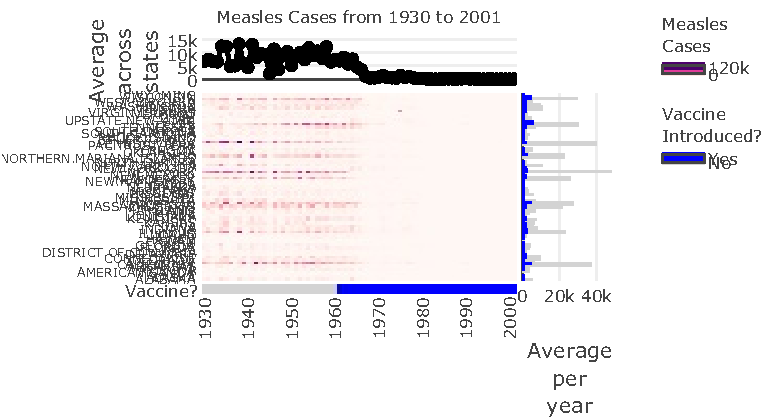
\includegraphics{R-data-viz_files/figure-latex/heatmap-demo-1.pdf}

Note that \texttt{iheatmapr} has a
\href{https://bioconductor.org}{Bioconductor} dependency, so if you have
never installed a package from Bioconductor before you will need to
install BiocInstaller first:

\begin{Shaded}
\begin{Highlighting}[]
\KeywordTok{source}\NormalTok{(}\StringTok{"https://bioconductor.org/biocLite.R"}\NormalTok{)}
\KeywordTok{biocLite}\NormalTok{(}\StringTok{"BiocInstaller"}\NormalTok{)}
\end{Highlighting}
\end{Shaded}

\section{\texorpdfstring{Networks (e.g.
\textbf{\texttt{visNetwork}})}{Networks (e.g. visNetwork)}}\label{networks-e.g.-visnetwork}

\href{https://CRAN.R-project.org/package=visNetwork}{\textbf{\texttt{visNetwork}}}
is an R interface to the \href{http://visjs.org/}{`vis.js' JavaScript
library}, a package to visualize networks in an interactive fashion. It
takes a table of nodes (vertices) and a table of edges (links) as
inputs. The example below is taken from
\href{http://kateto.net/network-visualization}{Katherine Ognyanova's
tutorial} and represents a network of hyperlinks and mentions among
various news sources.

\begin{Shaded}
\begin{Highlighting}[]
\KeywordTok{library}\NormalTok{(}\StringTok{'visNetwork'}\NormalTok{) }
\NormalTok{nodes <-}\StringTok{ }\KeywordTok{read.csv}\NormalTok{(}\StringTok{"https://github.com/cengel/R-data-viz/raw/master/demo-data/network/Dataset1-Media-Example-NODES.csv"}\NormalTok{, }\DataTypeTok{header=}\NormalTok{T, }\DataTypeTok{as.is=}\NormalTok{T)}
\NormalTok{links <-}\StringTok{ }\KeywordTok{read.csv}\NormalTok{(}\StringTok{"https://github.com/cengel/R-data-viz/raw/master/demo-data/network/Dataset1-Media-Example-EDGES.csv"}\NormalTok{, }\DataTypeTok{header=}\NormalTok{T, }\DataTypeTok{as.is=}\NormalTok{T)}
\NormalTok{nodes}\OperatorTok{$}\NormalTok{shape <-}\StringTok{ "dot"}  
\NormalTok{nodes}\OperatorTok{$}\NormalTok{shadow <-}\StringTok{ }\OtherTok{TRUE} \CommentTok{# Nodes will drop shadow}
\NormalTok{nodes}\OperatorTok{$}\NormalTok{title <-}\StringTok{ }\NormalTok{nodes}\OperatorTok{$}\NormalTok{media }\CommentTok{# Text on click}
\NormalTok{nodes}\OperatorTok{$}\NormalTok{label <-}\StringTok{ }\NormalTok{nodes}\OperatorTok{$}\NormalTok{type.label }\CommentTok{# Node label}
\NormalTok{nodes}\OperatorTok{$}\NormalTok{size <-}\StringTok{ }\NormalTok{nodes}\OperatorTok{$}\NormalTok{audience.size }\CommentTok{# Node size}
\NormalTok{nodes}\OperatorTok{$}\NormalTok{borderWidth <-}\StringTok{ }\DecValTok{2} \CommentTok{# Node border width}

\NormalTok{nodes}\OperatorTok{$}\NormalTok{color.background <-}\StringTok{ }\KeywordTok{c}\NormalTok{(}\StringTok{"slategrey"}\NormalTok{, }\StringTok{"tomato"}\NormalTok{, }\StringTok{"gold"}\NormalTok{)[nodes}\OperatorTok{$}\NormalTok{media.type]}
\NormalTok{nodes}\OperatorTok{$}\NormalTok{color.border <-}\StringTok{ "black"}
\NormalTok{nodes}\OperatorTok{$}\NormalTok{color.highlight.background <-}\StringTok{ "orange"}
\NormalTok{nodes}\OperatorTok{$}\NormalTok{color.highlight.border <-}\StringTok{ "darkred"}

\KeywordTok{visNetwork}\NormalTok{(nodes, links) }\OperatorTok
\StringTok{  }\KeywordTok{visOptions}\NormalTok{(}\DataTypeTok{highlightNearest =} \OtherTok{TRUE}\NormalTok{, }
             \DataTypeTok{selectedBy =} \StringTok{"type.label"}\NormalTok{)}
\end{Highlighting}
\end{Shaded}

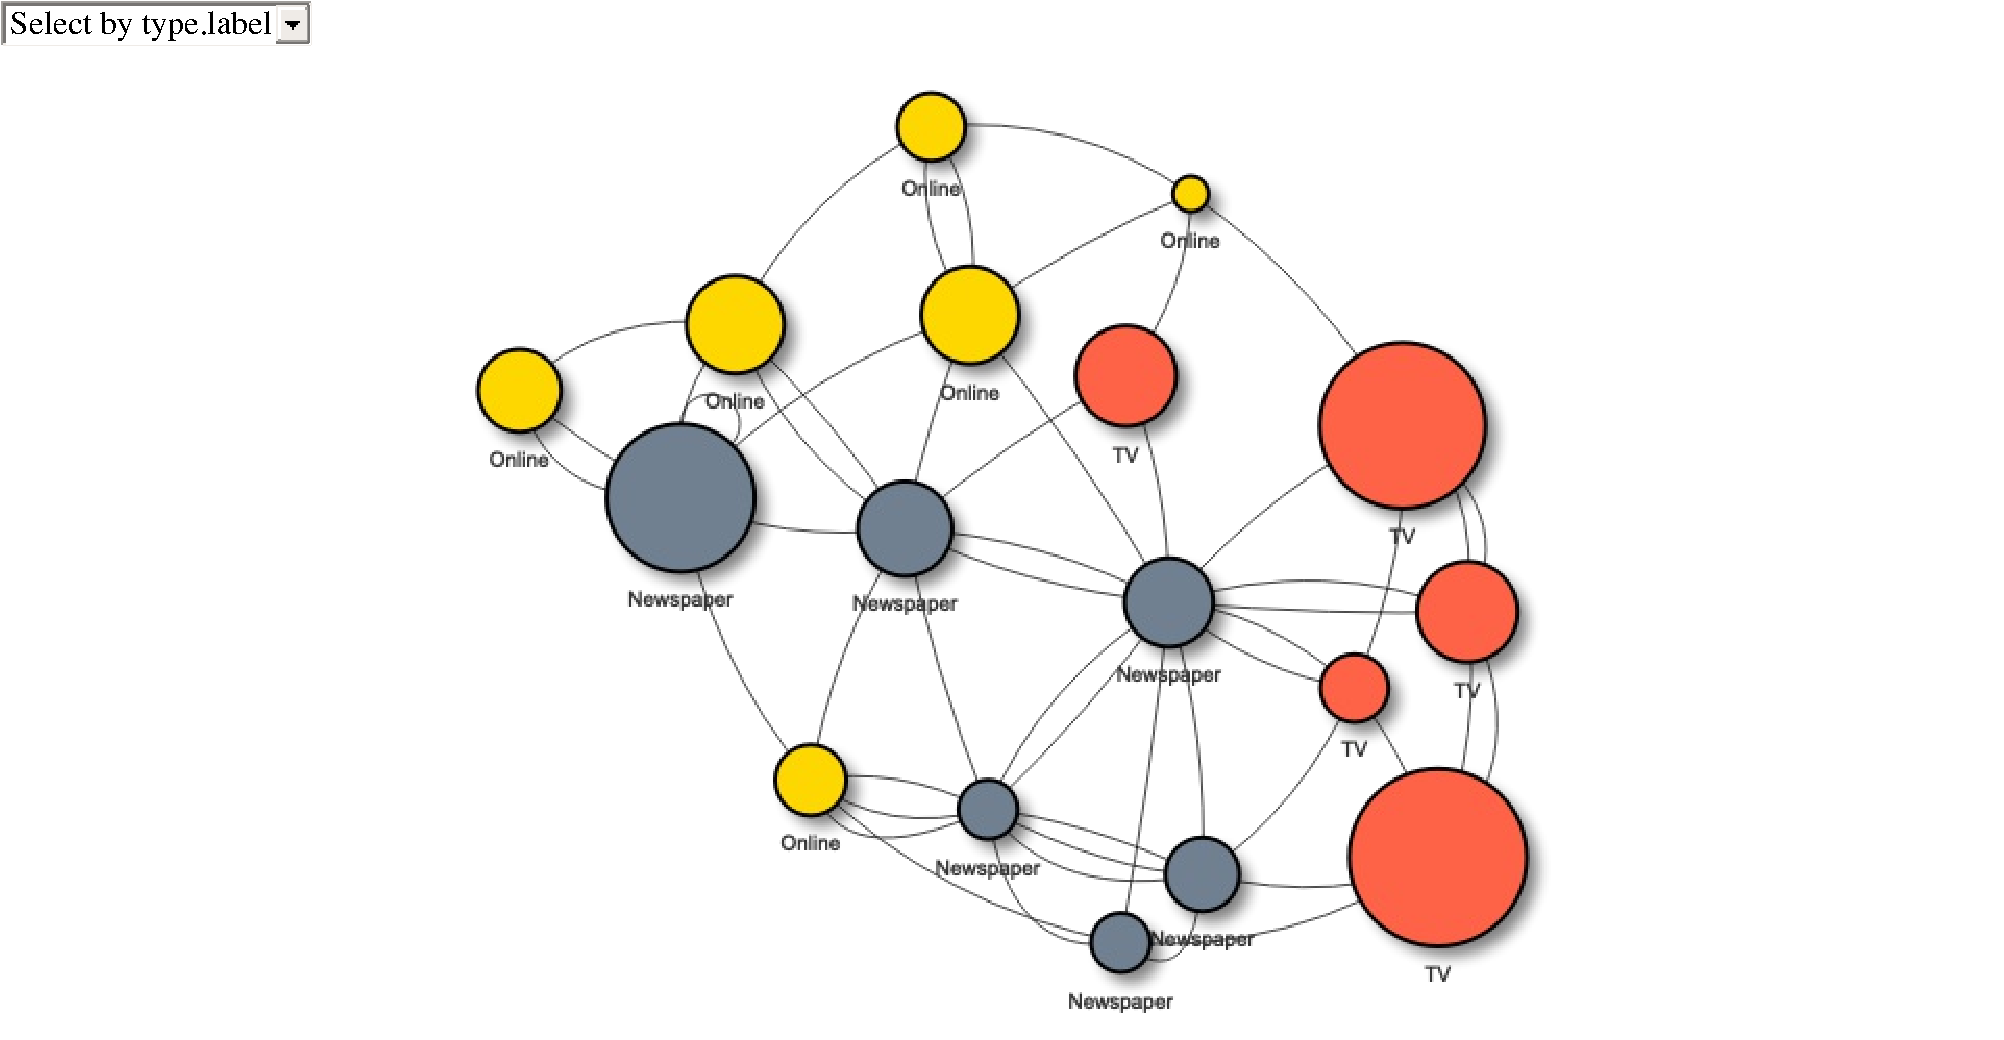
\includegraphics{R-data-viz_files/figure-latex/network-demo-1.pdf}

\section{\texorpdfstring{Maps (e.g.
\textbf{\texttt{tmap}})}{Maps (e.g. tmap)}}\label{maps-e.g.-tmap}

The
\href{https://CRAN.R-project.org/package=tmap}{\textbf{\texttt{tmap}}
package} is designed to visualize spatial data distributions in
geographic space, so called ``thematic maps''. The example is adapted
from
\href{https://github.com/mtennekes/tmap/tree/master/demo/LondonCrimes}{mtennekes}
and shows a map of crimes registered during October 2015. We combine
several layers, one with the outline of London, one with the river
Thames, and one with the actual crime densities.

For this demo we first need to download the data. If you have your
working directory set to \texttt{R-data-viz} and it contains a folder
called \texttt{data}, this will download and extract the map data into a
subfolder of your \texttt{data} folder, called \texttt{map}:

\begin{Shaded}
\begin{Highlighting}[]
\KeywordTok{download.file}\NormalTok{(}\StringTok{"https://github.com/cengel/R-data-viz/raw/master/demo-data/map.zip"}\NormalTok{,}
              \StringTok{"data/map.zip"}\NormalTok{)}
\KeywordTok{unzip}\NormalTok{(}\StringTok{"data/map.zip"}\NormalTok{, }\DataTypeTok{exdir=}\StringTok{"data"}\NormalTok{)}
\end{Highlighting}
\end{Shaded}

Now, here is the map.

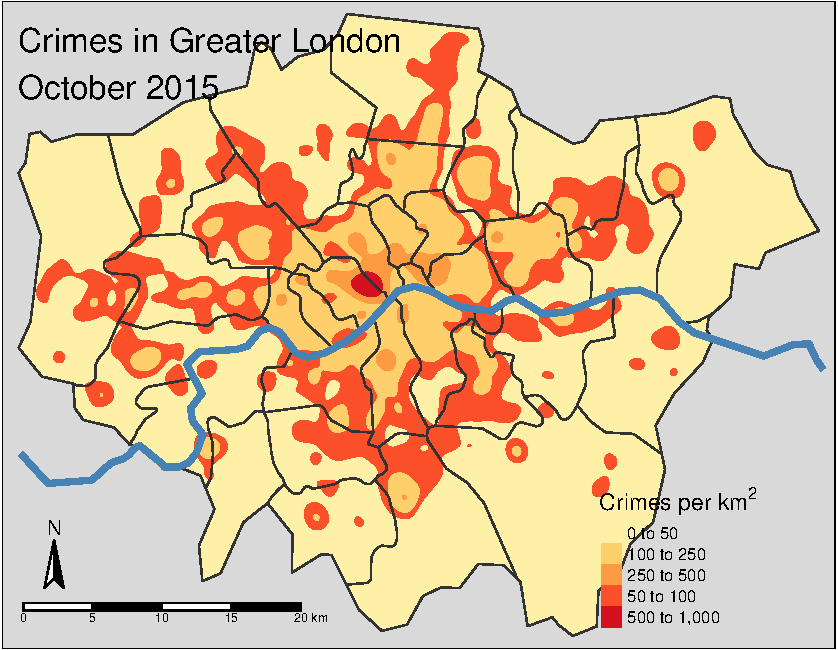
\includegraphics{R-data-viz_files/figure-latex/tmap-demo-1.pdf}

\begin{Shaded}
\begin{Highlighting}[]
\KeywordTok{library}\NormalTok{(tmap)}
\KeywordTok{library}\NormalTok{(tmaptools)}
\KeywordTok{suppressPackageStartupMessages}\NormalTok{(}\KeywordTok{library}\NormalTok{(sf))}
              
\NormalTok{london <-}\StringTok{ }\KeywordTok{st_read}\NormalTok{(}\StringTok{"data/map"}\NormalTok{, }\StringTok{"London"}\NormalTok{, }\DataTypeTok{quiet =} \OtherTok{TRUE}\NormalTok{)}
\NormalTok{crime_densities <-}\StringTok{ }\KeywordTok{st_read}\NormalTok{(}\StringTok{"data/map"}\NormalTok{, }\StringTok{"Crimes"}\NormalTok{, }\DataTypeTok{quiet =} \OtherTok{TRUE}\NormalTok{)}
\NormalTok{thames <-}\StringTok{ }\KeywordTok{st_read}\NormalTok{(}\StringTok{"data/map"}\NormalTok{, }\StringTok{"Thames"}\NormalTok{, }\DataTypeTok{quiet =} \OtherTok{TRUE}\NormalTok{)}

\KeywordTok{tm_shape}\NormalTok{(crime_densities) }\OperatorTok{+}
\StringTok{  }\KeywordTok{tm_fill}\NormalTok{(}\DataTypeTok{col =} \StringTok{"level"}\NormalTok{, }\DataTypeTok{palette =} \StringTok{"YlOrRd"}\NormalTok{, }
    \DataTypeTok{title =} \KeywordTok{expression}\NormalTok{(}\StringTok{"Crimes per "} \OperatorTok{*}\StringTok{ }\NormalTok{km}\OperatorTok{^}\DecValTok{2}\NormalTok{)) }\OperatorTok{+}\StringTok{ }
\KeywordTok{tm_shape}\NormalTok{(london) }\OperatorTok{+}\StringTok{ }\KeywordTok{tm_borders}\NormalTok{() }\OperatorTok{+}
\KeywordTok{tm_shape}\NormalTok{(thames) }\OperatorTok{+}\StringTok{ }\KeywordTok{tm_lines}\NormalTok{(}\DataTypeTok{col =} \StringTok{"steelblue"}\NormalTok{, }\DataTypeTok{lwd =} \DecValTok{4}\NormalTok{) }\OperatorTok{+}
\KeywordTok{tm_compass}\NormalTok{(}\DataTypeTok{position =} \KeywordTok{c}\NormalTok{(}\StringTok{"left"}\NormalTok{, }\StringTok{"bottom"}\NormalTok{)) }\OperatorTok{+}
\KeywordTok{tm_scale_bar}\NormalTok{(}\DataTypeTok{position =} \KeywordTok{c}\NormalTok{(}\StringTok{"left"}\NormalTok{, }\StringTok{"bottom"}\NormalTok{)) }\OperatorTok{+}\StringTok{ }
\KeywordTok{tm_style_gray}\NormalTok{(}\DataTypeTok{title =} \StringTok{"Crimes in Greater London}\CharTok{\textbackslash{}n}\StringTok{October 2015"}\NormalTok{)}
\end{Highlighting}
\end{Shaded}

Good starting places to look for additional examples and packages are
the R Graph Gallery: \url{https://www.r-graph-gallery.com/all-graphs/}
and the CRAN Task View: \url{https://CRAN.R-project.org/view=Graphics}.

\bibliography{book.bib,packages.bib}


\end{document}
